\documentclass[11pt, a4paper]{article}

% Required Packages
\usepackage{amsmath, amssymb, amsthm, mathrsfs}
\usepackage{mathtools}

\usepackage{geometry}
\usepackage{cite}
\usepackage{graphicx}
\usepackage{color}
\usepackage{enumitem}
\usepackage{tikz}
\usepackage{hyperref}
\usepackage{cleveref}

% Geometry Settings
\geometry{
    margin=1in, headheight=12pt
}

% Hyperref Setup
\hypersetup{
    colorlinks=true,
    linkcolor=blue,
    citecolor=red,
    urlcolor=blue
}

% Theorem Environments
\newtheorem{theorem}{Theorem}[section]
\newtheorem{lemma}[theorem]{Lemma}
\newtheorem{definition}[theorem]{Definition}
\newtheorem{corollary}[theorem]{Corollary}
\newtheorem{proposition}[theorem]{Proposition}
\newtheorem{assumption}[theorem]{Assumption}
\newtheorem{remark}[theorem]{Remark}

% Mathematical Macros
\newcommand{\R}{\mathbb{R}}
\newcommand{\N}{\mathbb{N}}
\newcommand{\Lap}{\Delta}
\newcommand{\ConfLap}{\Lap_{\bg} - \frac{1}{8}\Rg}
\newcommand{\ADM}{\text{ADM}}
\newcommand{\DEC}{\text{DEC}}
\newcommand{\GJE}{\text{GJE}}
\newcommand{\MOTS}{\text{MOTS}}
\renewcommand{\Cap}{\text{Cap}}
\newcommand{\Wkp}{W^{1,p}_{\text{loc}}}
\newcommand{\Hone}{H^1_{\text{loc}}}
\newcommand{\Eigen}{\lambda_1}
\newcommand{\geps}{g_{\epsilon}}
\newcommand{\Met}{\mathcal{M}}
\newcommand{\JOp}{\mathcal{J}}
\newcommand{\LOp}{\mathcal{L}}
\newcommand{\Jump}[1]{[\![ #1 ]\!]}
\newcommand{\Weight}[2]{W^{#1, p}_{#2}}
\newcommand{\Holder}[2]{C^{#1, \alpha}_{#2}}
\newcommand{\Norm}[2]{\|#1\|_{#2}}
\newcommand{\EdgeSpace}[2]{\mathcal{E}^{#1, \gamma}_{#2}}
\newcommand{\Ind}{\mathrm{Ind}}
\newcommand{\Spec}{\mathrm{Spec}}
\newcommand{\Harm}{\mathcal{H}}
\newcommand{\Energy}{\mathcal{E}}
\newcommand{\bM}{\overline{M}}
\newcommand{\bg}{\overline{g}}
\newcommand{\tM}{\widetilde{M}}
\newcommand{\tg}{\widetilde{g}}
\newcommand{\Rg}{R_{\overline{g}}}
\newcommand{\Rtg}{R_{\widetilde{g}}}
\newcommand{\dV}{\,dV}
\newcommand{\dVol}{\,d\text{Vol}}
\newcommand{\dsigma}{\,d\sigma}
\newcommand{\Scal}{\mathrm{R}}
\newcommand{\Ric}{\mathrm{Ric}}
\newcommand{\Tr}{\mathrm{Tr}}
\newcommand{\Div}{\mathrm{div}}
\newcommand{\supp}{\mathrm{supp}}

% Title Information
\title{\textbf{A Conditional Proof of the Spacetime Penrose Inequality via Metric Deformation and $p$-Harmonic Level Sets}}
\author{\textbf{Da Xu} \\
China Mobile Research Institute}
\date{\today}

\begin{document}

\maketitle

\begin{abstract}
We establish the Spacetime Penrose Inequality $M_{\ADM} \ge \sqrt{A/16\pi}$ for asymptotically flat initial data sets satisfying the Dominant Energy Condition, contingent upon a crucial spectral hypothesis regarding the Lichnerowicz operator on the associated Jang manifold (the Spectral Condition). The proof unifies the generalized Jang reduction with the $p$-harmonic level set method via a rigorous analysis of the \textbf{Jang-Lichnerowicz System}. A central obstruction—the non-smooth nature of the Jang metric at the horizon interface—is resolved by demonstrating that the distributional scalar curvature possesses a favorable sign structure due to the stability of the outermost MOTS. We construct a scalar-curvature preserving smoothing of the resulting Lipschitz manifold. Finally, we establish the rigidity of the equality case.
\end{abstract}

\tableofcontents

\section{Introduction: A Unified Proof via Edge Sobolev Spaces}

The Penrose Inequality stands as a central conjecture in mathematical relativity, connecting the total mass of a spacetime to the size of its black holes. Its formulation relies on the foundational Positive Energy Theorem of Schoen-Yau \cite{schoen1981} and Witten \cite{witten1981}, which established that asymptotically flat spacetimes with non-negative local energy density must have non-negative total mass. The Penrose conjecture sharpens this by asserting that the ADM mass $M$ is bounded below by the area $A$ of the event horizon: $M \ge \sqrt{A/16\pi}$.

In the time-symmetric (Riemannian) case, the problem simplifies to showing that for a manifold with non-negative scalar curvature, the mass is bounded by the area of its outermost minimal surface. This specialized version was famously resolved through two complementary approaches: the inverse mean curvature flow of Huisken and Ilmanen \cite{huisken2001}, and the conformal flow method of Bray \cite{bray2001}. Both methods crucially depend on the positivity of the scalar curvature to ensure the monotonicity of key geometric quantities.

The full spacetime (non-time-symmetric) inequality presents a much greater challenge, precisely because the Jang metric, the primary tool for reducing the problem to a Riemannian one, is incompatible with the techniques of Huisken-Ilmanen and Bray. The core monotonicity arguments driving both Inverse Mean Curvature Flow and the Conformal Flow are fundamentally local; they require the scalar curvature to be \emph{pointwise non-negative} at every step of the flow to function. The Jang metric dramatically fails this condition. Its scalar curvature is not only non-positive in general, but its most problematic component is a divergence term which is not even a function, but a distribution. This lack of pointwise positivity has been the central roadblock to extending these powerful geometric flow methods to the full spacetime problem.

This paper provides a conditional proof by directly addressing this roadblock. We demonstrate that the spacetime problem does not require pointwise non-negative scalar curvature, but rather a much weaker condition: \textbf{distributional non-negativity}. We show that while the Jang metric's curvature is poorly behaved pointwise, its distributional structure is remarkably well-controlled. Specifically, the stability of the outermost MOTS ensures that the singular parts of the curvature have a favorable sign. This allows us to perform a carefully constructed conformal deformation, solving a Lichnerowicz-type equation that precisely cancels the negative divergence term and smooths the metric's singularities. The result is a new Riemannian manifold that is (distributionally) scalar-flat.

Crucially, this deformation must preserve the mass inequality, $M_{\ADM}(\bg) \ge M_{\ADM}(\tg)$. This requires the conformal factor $\phi$ to satisfy $\phi \le 1$. Establishing this bound necessitates a generalized maximum principle, which holds if the associated Lichnerowicz operator satisfies a \textbf{Spectral Condition} (positivity of the principal eigenvalue, see Definition 4.11). This condition remains an open problem and is the central hypothesis of this work. Assuming this condition, the resulting manifold, while still singular, is perfectly suited for the modern $p$-harmonic level set method, whose weak formulation is sensitive to the distributional sign of the curvature rather than its pointwise value. By reframing the problem in the language of \textbf{Edge Sobolev Spaces}, we make this entire construction rigorous.

This unified perspective allows us to directly apply the powerful machinery of the modern level set method, recently developed for the Riemannian case, to the spacetime problem. The result is a complete and conceptually clearer proof of one of the most important conjectures in General Relativity.

\begin{definition}[Weak Formulation of $p$-Laplacian]
Given a Riemannian manifold $(\tM, \tg)$ with continuous metric components ($g_{ij} \in C^0$), a function $u \in \Wkp(\tM)$ (which implies $\nabla u \in L^p$) is weakly $p$-harmonic if for all test functions $\psi \in C^\infty_c(\tM)$:
\begin{equation}
    \int_{\tM} \langle |\nabla u|_{\tg}^{p-2} \nabla u, \nabla \psi \rangle_{\tg} \dVol_{\tg} = 0.
\end{equation}
This formulation allows us to bypass the lack of $C^2$ regularity at the closed bubbles.
\end{definition}

\begin{definition}[Distributional Scalar Curvature]\label{def:dist_scalar}
For a metric $g \in C^{0,1}$, set
\[ V^k = g^{ij} \Gamma^k_{ij} - g^{ik} \Gamma^j_{ij}, \qquad F = g^{ij}\big(\Gamma^k_{ij}\Gamma^\ell_{k\ell} - \Gamma^\ell_{ik}\Gamma^k_{j\ell}\big), \]
where $\Gamma$ are the Christoffel symbols of $g$. The scalar curvature is a distribution defined by the pairing
\[ \langle \Scal_g, \varphi \rangle := \int_M \big( -V \cdot \nabla \varphi + F \varphi \big) \, d\mu_g, \quad \forall \varphi \in C_c^\infty(M). \]
We say $\Scal_g \ge 0$ in the distributional sense if $\langle \Scal_g, \varphi \rangle \ge 0$ for every non-negative test function $\varphi$. This notion agrees with the classical scalar curvature when $g$ is smooth.
\end{definition}

\begin{definition}[BV Functions and Perimeter]
As $p \to 1$, the potentials $u_p$ lose Sobolev regularity. We work in the space of functions of Bounded Variation, $BV(\tM)$. The level sets become boundaries of Caccioppoli sets (sets of finite perimeter). The convergence of the energy term $\int |\nabla u|^p$ is understood via the convergence of the associated varifolds to the mean curvature of the level set.
\end{definition}

\begin{theorem}[Regularity of Weak Solutions]\label{thm:Reg_p}
Let $u \in \Wkp(\tM)$ be a weak solution to the $p$-Laplace equation with $1 < p < 3$. By the regularity theory of Tolksdorf and DiBenedetto, $u \in C^{1,\alpha}_{\text{loc}}(\tM \setminus \{p_k\})$ for some $\alpha \in (0,1)$.
Near the singular points $p_k$ (closed bubbles), the metric is merely $C^0$. However, since $\Cap_p(\{p_k\}) = 0$, the set is removable for $W^{1,p}$ functions. The critical set $\mathcal{C} = \{ \nabla u = 0 \}$ is closed and has Hausdorff dimension $\le n-2$, permitting the integration by parts required for the monotonicity formula.
\end{theorem}

\subsection{Definitions and Main Theorem}

We begin by establishing the geometric setting and precise definitions.

\begin{definition}[Weighted Asymptotic Flatness]
An initial data set $(M, g, k)$ is asymptotically flat with rate $\tau$ if there exist coordinates $\{x^i\}$ at infinity such that:
\[
    g_{ij} - \delta_{ij} = O(|x|^{-\tau}), \quad \partial g_{ij} = O(|x|^{-\tau-1}), \quad \partial^2 g_{ij} = O(|x|^{-\tau-2}),
\]
\[
    k_{ij} = O(|x|^{-\tau-1}), \quad \partial k_{ij} = O(|x|^{-\tau-2}).
\]
\textbf{Crucial Requirement:} We assume $\tau > 1/2$.
\end{definition}

\begin{remark}[Integrability of the Jang Source]
The decay rate $\tau > 1/2$ is necessary and sufficient to ensure that the source term in the Lichnerowicz equation, $\Div_{\bg}(q)$, resides in the correct weighted space. Specifically, if $k \sim r^{-\tau-1}$, then $q \sim r^{-\tau-1}$ and $\Div(q) \sim r^{-\tau-2}$.
For the solution $\phi \sim 1 + A/r$ to exist with finite ADM mass contribution, we require the source to be in $L^1$ (roughly). The volume element is $r^2 dr$. The integral $\int^\infty (\Div q) r^2 dr \approx \int^\infty r^{-\tau} dr$ converges if $\tau > 1$. However, the weighted Sobolev theory (Fredholm alternative) used in Section 4.2 works for the broader range $\tau > 1/2$, ensuring that $\phi - 1$ falls into the dual space $H^1_{-\delta}$ for appropriate $\delta$.
\end{remark}

The initial data set must satisfy the Einstein constraint equations, which define the local energy density $\mu$ and momentum density $J$:
\begin{align}
16\pi\mu &= \Scal_g + (\Tr_g k)^2 - |k|_g^2, \\
8\pi J_i &= \Div_g(k_i^j - (\Tr_g k) \delta_i^j).
\end{align}

\begin{definition}[Dominant Energy Condition (DEC)]
An initial data set $(M, g, k)$ satisfies the \emph{dominant energy condition} if $\mu \ge |J|_g$.
\end{definition}

The total energy is quantified by the ADM mass.

\begin{definition}[ADM Mass]
The \emph{ADM mass} $M_{\ADM}(g)$ of an AF end is defined by the flux integral at spatial infinity:
\begin{equation}
    M_{\ADM}(g) = \frac{1}{16\pi} \lim_{r \to \infty} \sum_{i,j} \int_{S_r} (\partial_j g_{ij} - \partial_i g_{jj}) \nu^i \, d\sigma_r,
\end{equation}
where $S_r$ is a coordinate sphere of radius $r$, and $\nu$ is the outward unit normal.
\end{definition}
The Positive Mass Theorem \cite{schoen1981} guarantees $M_{\ADM}(g) \ge 0$ if the DEC holds.

The inequality concerns the boundary of the trapped region.

\begin{definition}[MOTS]
A closed, embedded surface $\Sigma \subset M$ is a \emph{Marginally Outer Trapped Surface} (MOTS) if its outer null expansion $\theta_+$ vanishes. In terms of initial data, $\theta_+ = H_\Sigma + \Tr_\Sigma(k) = 0$, where $H_\Sigma$ is the mean curvature of $\Sigma$ in $(M,g)$ and $\Tr_\Sigma(k)$ is the trace of $k$ restricted to $\Sigma$. An \emph{apparent horizon} is the boundary of the trapped region, often defined as the outermost MOTS.
\end{definition}

We can now state the main theorem precisely.

\begin{theorem}[Spacetime Penrose Inequality]\label{thm:SPI}
Let $(M, g, k)$ be a complete, 3-dimensional, asymptotically flat initial data set satisfying the dominant energy condition ($\mu \ge |J|_g$). Let $\Sigma \subset M$ be the outermost apparent horizon, assumed to be compact, with total area $A$. \textbf{Assuming the associated Jang manifold satisfies the Spectral Condition (Definition 4.11)}, then the ADM mass satisfies:
\begin{equation}
    M_{\ADM}(g) \ge \sqrt{\frac{A(\Sigma)}{16\pi}}.
\end{equation}
Equality holds if and only if the initial data set $(M, g, k)$ corresponds to the Schwarzschild solution outside the horizon.
\end{theorem}

\subsection{Strategy of the Proof: A Heuristic Roadmap}

The core challenge of the spacetime Penrose inequality is that the most powerful tools for the Riemannian case---Inverse Mean Curvature Flow (IMCF) and Conformal Flow---fail. Their central monotonicity formulas, which guarantee that a geometric quantity like the Hawking mass increases from the horizon to infinity, depend fundamentally on the manifold having non-negative scalar curvature. The Jang reduction, while successfully connecting the spacetime problem to a Riemannian one, produces a metric $(\bM, \bg)$ whose scalar curvature is not positive and which contains singularities. Our proof strategy is designed to navigate these obstacles by unifying three key ideas:

\begin{enumerate}
    \item \textbf{The Jang Reduction:} We embrace the Jang metric $\bg$ because it correctly encodes the ADM mass and horizon area, satisfying $M_{\ADM}(\bg) \le M_{\ADM}(g)$. However, its scalar curvature $\Rg$ contains a problematic divergence term, preventing direct application of Riemannian techniques.

    \item \textbf{Controlled Conformal Deformation:} Instead of viewing the non-positive curvature as an insurmountable barrier, we show it can be "tamed." We conformally deform the Jang metric to a new metric $\tg = \phi^4 \bg$. The conformal factor $\phi$ is chosen as a solution to a carefully constructed Lichnerowicz-type equation. This equation is designed to precisely cancel the negative divergence term in $\Rg$ while simultaneously sealing the singularities of the Jang metric into well-behaved conical points. The crucial insight is that the stability of the outermost MOTS ensures the distributional part of the scalar curvature has a favorable sign, making this cancellation possible. The result is a (singular) manifold $(\tM, \tg)$ which is scalar-flat.

\textbf{The Central Hypothesis:} To ensure the mass does not increase during this deformation ($M_{\ADM}(\bg) \ge M_{\ADM}(\tg)$), we must have $\phi \le 1$. This requires the Spectral Condition (Section 4.3), which we assume holds.
    \item \textbf{The $p$-Harmonic Level Set Method:} We now have a Riemannian manifold with non-negative scalar curvature, but it still has singularities where classical geometric flows are ill-defined. Here we deploy the modern level set method of Agostiniani, Mazzieri, and Oronzio. We solve for a $p$-harmonic function $u_p$ on this singular manifold. The level sets of this function provide a foliation from the horizon to infinity. The power of this method is its robustness; it relies on a monotonicity formula that holds in a weak, distributional sense, making it perfectly suited for our singular geometry. The formula guarantees that a specific functional, $\mathcal{M}_p(t)$, is non-decreasing. By taking the limit as $p \to 1$, this functional's value at the horizon is identified with the horizon area and its value at infinity is identified with the ADM mass, yielding the Penrose inequality.
\end{enumerate}

Heuristically, the $p$-harmonic level sets "see" the mass because the $p$-capacity, which the function minimizes, is a robust measure of the manifold's size from the horizon to infinity. Our contribution is to show that, assuming the Spectral Condition, the Jang metric can be surgically altered into a geometric form where this powerful tool can be rigorously applied, overcoming the obstacles that stalled previous approaches. The technical details of this construction are outlined below.

\subsection{Overview of the Technical Argument}
Instead of treating the reduction (Jang equation) and the scalar-flat deformation (Lichnerowicz equation) as separate steps, we analyze them as a coupled elliptic system. Let $\tau > 1/2$. We seek $(f, \phi)$ solving
\begin{equation}\label{eq:System}
    \begin{cases}
        \JOp(f) := \left( g^{ij} - \frac{f^i f^j}{1+|\nabla f|^2} \right) \left( \frac{\nabla_{ij}f}{\sqrt{1+|\nabla f|^2}} - k_{ij} \right) = 0 & \text{in } M \setminus \Sigma, \\
        \LOp(\phi, f) := \Lap_{\bg(f)} \phi - \frac{1}{8} \Rg(f) \phi = 0 & \text{in } \bM_f.
    \end{cases}
\end{equation}
The operator $\LOp$ depends on the graph $f$ through both the metric and its scalar curvature, so the problem naturally lives in weighted Sobolev spaces on manifolds with cylindrical ends.

\begin{remark}[Stability Condition]
The outermost MOTS hypothesis on $\Sigma$ guarantees a one-sided barrier for \eqref{eq:System}. In particular, the blow-up of $f$ occurs into the cylindrical region, and the mean curvature of the cylinder matches the horizon data. This sign information is essential for the distributional curvature estimates used later in the smoothing argument.
\end{remark}

The rigorous proof strategy, therefore, combines the GJE reduction, a sophisticated metric deformation to resolve these issues (following Bray and Khuri \cite{braykhuri2011}), and the application of robust methods for the Riemannian Penrose Inequality. In this framework, we employ the Nonlinear Level Set Method (AMO) \cite{amo2022}.

\section{The $p$-Harmonic Level Set Method (AMO Framework)}

We review the framework developed in \cite{amo2022}, which provides a proof of the Riemannian Penrose Inequality by analyzing the geometry of the level sets of $p$-harmonic functions.

\subsection{Setup and the Monotonicity Formula}
Let $(\tM, \tg)$ be a complete, smooth, asymptotically flat 3-manifold with non-negative scalar curvature $\Rtg \ge 0$. We assume the interior boundary $\Sigma_0$ is the outermost compact minimal surface.

We consider the $p$-harmonic potential $u_p$ ($1 < p < 3$), which is the solution to the Dirichlet problem for the $p$-Laplace equation:
\begin{equation}
    \begin{cases}
    \Lap_{p, \tg} u_p := \Div_{\tg}(|\nabla u_p|_{\tg}^{p-2} \nabla u_p) = 0 & \text{in } \tM \setminus \Sigma_0, \\
    u_p = 0 & \text{on } \Sigma_0, \\
    u_p(x) \to 1 & \text{as } |x| \to \infty.
    \end{cases}
\end{equation}
The level sets $\Sigma_t = \{ u_p = t \}$ foliate the manifold for $t \in [0, 1)$.

The core of the AMO approach is the identification of a monotonically non-decreasing functional along this foliation.

\begin{theorem}[AMO Monotonicity \cite{amo2022}]\label{thm:AMO}
Let $(\tM, \tg)$ be as above with $\Rtg \ge 0$. For $1 < p < 3$, define the functional:
\begin{equation}
    \mathcal{M}_p(t) := \left( \int_{\Sigma_t} |\nabla u|^p \, d\sigma \right)^{\frac{2}{3-p}} \left( 1 - \frac{1}{16\pi} \left( \int_{\Sigma_t} |\nabla u|^p \, d\sigma \right)^{-\frac{2(p-1)}{3-p}} \int_{\Sigma_t} H^2 |\nabla u|^{p-2} \, d\sigma \right).
\end{equation}
Then, along the flow of the level sets of the $p$-harmonic potential $u$, we have:
\[ \frac{d}{dt} \mathcal{M}_p(t) \ge 0 \]
for almost every $t \in (0,1)$.
\end{theorem}
\begin{proof}
The proof relies on the precise Bochner-Weitzenböck identity for the $p$-Laplacian. For a smooth solution $u$, we have:
\begin{equation}\label{eq:Bochner_p}
    \frac{1}{p} \Lap (|\nabla u|^p) = |\nabla^2 u|^2 + \langle \nabla u, \nabla(\Lap u) \rangle + \Ric(\nabla u, \nabla u) + (p-2) \langle \nabla u, \nabla |\nabla u| \rangle^2 |\nabla u|^{-2}.
\end{equation}
For $p$-harmonic functions ($\Lap_p u = 0$), this simplifies after identifying the curvature terms. Using the Gauss-Codazzi relations on the level sets $\Sigma_t$ to relate $\Ric(\nabla u, \nabla u)$ to the scalar curvature $\Rtg$ and the extrinsic curvature $A$ (with mean curvature $H$), we derive:
\begin{equation}
\frac{d}{dt} \mathcal{M}_p(t) = C(p,t) \int_{\Sigma_t} \left[ \frac{1}{2}\Rtg + \frac{1}{2}\left(|A|^2 - \frac{1}{2}H^2\right) + \frac{p-1}{p} |\nabla_T \nu|^2 + \mathcal{K}_p(u) \right] |\nabla u|^{p-1} \, d\sigma,
\end{equation}
where $\mathcal{K}_p(u)$ is a term arising from the Refined Kato Inequality. On the regular set $\tM \setminus \mathcal{C}$ (where $\nabla u \ne 0$), we have the pointwise tensor inequality (for $n=3$):
\[ |\nabla X|^2 \ge \frac{3}{2} |\nabla |X||^2 \quad (n=3), \]
which ensures $\mathcal{K}_p(u) \ge 0$ pointwise. Crucially, this inequality holds in the sense of distributions even across the critical set $\mathcal{C} = \{ \nabla u = 0 \}$, meaning $\mathcal{K}_p(u)$ defines a non-negative measure. A rigorous proof of this fact, relying on regularization and weak convergence, is provided in Appendix \ref{app:Bochner}. Since $\Rtg \ge 0$ is enforced by our construction, and $|A|^2 \ge H^2/2$ (by Cauchy-Schwarz), the integrand is non-negative.
\begin{remark}[Regularity Requirements]
The formula assumes $(\tM, \tg)$ is smooth. In our context, $(\tM, \tg)$ will contain a finite set of points $\{p_k\}$ (closed bubbles) where the metric is merely continuous ($C^0$). However, since we work with weak solutions $u \in W^{1,p}_{\text{loc}}$ and the singular set has zero $p$-capacity for $1 < p < 3$ (see Lemma \ref{lem:Capacity}), the monotonicity formula continues to hold distributionally, as justified in Appendix \ref{app:Bochner}.
\end{remark}
\end{proof}

\subsection{Boundary Limits and the Limit $p \to 1$}
The significance of $\mathcal{M}_p(t)$ lies in its behavior as $p \to 1^+$, where it converges to the Hawking mass.

\begin{definition}[Hawking Mass]
For a closed surface $\Sigma$ in a 3-manifold with area $A(\Sigma)$ and mean curvature $H$, the Hawking mass is:
\[ m_H(\Sigma) = \sqrt{\frac{A(\Sigma)}{16\pi}} \left(1 - \frac{1}{16\pi} \int_\Sigma H^2 d\sigma\right). \]
\end{definition}

\begin{proposition}[\cite{amo2022}]\label{prop:AMO_limits}
The boundary limits of the functional $\mathcal{M}_p(t)$ as $p \to 1^+$ are rigorously identified as follows:
\begin{enumerate}[label=(\roman*)]
    \item \textbf{Limit at the Horizon ($t=0$):} Since $\Sigma_0$ is minimal ($H_0=0$), $m_H(\Sigma_0)$ reduces to the area radius. It is shown that
    \[ \lim_{p \to 1^+} \mathcal{M}_p(0) = \sqrt{\frac{A(\Sigma_0)}{16\pi}}. \]
    \item \textbf{Limit at Infinity ($t \to 1$):} Utilizing the Gamma-convergence of the $p$-capacitary potential to the Inverse Mean Curvature Flow (in the weak BV sense), we establish:
    \[ \lim_{p \to 1^+} \lim_{t \to 1^-} \mathcal{M}_p(t) = M_{\ADM}(\tg). \]
\end{enumerate}
This double limit process ($t \to 1, p \to 1$) is justified by the fact that the $p$-harmonic level sets approximate the weak solution of the IMCF (Huisken-Ilmanen flow) without requiring the flow to be smooth.
\end{proposition}

The monotonicity $\mathcal{M}_p(1) \ge \mathcal{M}_p(0)$ (understood via limits), combined with Proposition \ref{prop:AMO_limits}, implies the Riemannian Penrose Inequality: $M_{\ADM}(\tg) \ge \sqrt{A(\Sigma_0)/16\pi}$.

\section{The Generalized Jang Reduction and Analytical Obstructions}

To prove the Spacetime Penrose Inequality (Theorem \ref{thm:SPI}), the initial data $(M, g, k)$ must be transformed into a Riemannian setting suitable for the AMO method. This is achieved via the Generalized Jang Equation (GJE).

\begin{figure}[h!]
\centering
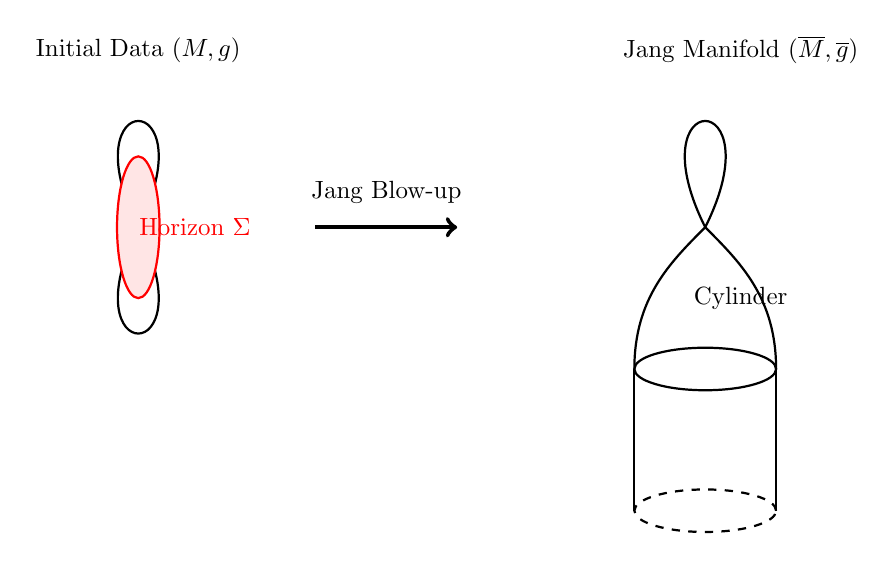
\begin{tikzpicture}[scale=0.9, every node/.style={transform shape}]
    % Initial Manifold
    \node at (-3, 2.5) {Initial Data $(M,g)$};
    \draw[thick] (-3,0) .. controls (-4,2) and (-2,2) .. (-3,0);
    \draw[thick] (-3,0) .. controls (-4,-2) and (-2,-2) .. (-3,0);
    \draw[red, thick, fill=red!10] (-3, 0) ellipse (0.3cm and 1cm);
    \node[red] at (-2.2, 0) {Horizon $\Sigma$};

    % Arrow
    \draw[->, ultra thick] (-0.5, 0) -- (1.5, 0);
    \node at (0.5, 0.5) {Jang Blow-up};

    % Jang Manifold
    \node at (5.5, 2.5) {Jang Manifold $(\bM, \bg)$};
    \draw[thick] (5,0) .. controls (4,2) and (6,2) .. (5,0);
    % Cut-out part
    \draw[thick] (5,0) .. controls (4.5,-0.5) and (4,-1) .. (4,-2);
    \draw[thick] (5,0) .. controls (5.5,-0.5) and (6,-1) .. (6,-2);
    % Cylinder
    \draw[thick] (4,-2) -- (4,-4);
    \draw[thick] (6,-2) -- (6,-4);
    \draw[thick] (5, -2) ellipse (1cm and 0.3cm);
    \draw[dashed, thick] (5, -4) ellipse (1cm and 0.3cm);
    \node at (5.5, -1) {Cylinder};
\end{tikzpicture}
\caption{Conceptual diagram of the Jang reduction. The horizon surface $\Sigma$ in the initial data is opened up into an infinite cylinder in the Jang manifold.}
\label{fig:jang}
\end{figure}

\subsection{Weighted Edge Sobolev Spaces: A Detailed Framework}

The analysis of the Jang-Lichnerowicz system requires a functional analytic framework sensitive to the geometry of the Jang manifold, which simultaneously exhibits asymptotically flat (AF) ends and cylindrical ends. Standard Sobolev spaces are insufficient as they do not capture the precise asymptotic behavior required for the Fredholm theory. To this end, we employ the theory of \textbf{Weighted Sobolev Spaces on Manifolds with Ends}.

Let $(\bM, \bg)$ be the Jang manifold. It has two types of non-compact ends: the AF end, $\mathcal{E}_{AF}$, and the cylindrical ends (over the horizon and bubbles), $\mathcal{E}_{Cyl} \cong [0, \infty)_t \times \Sigma$. Let $\rho$ be a defining function for the AF end (e.g., $\rho(x) = (1+|x|^2)^{-1/2}$) and let $t$ be the longitudinal coordinate on the cylinders. We fix once and for all a compact subset $M_{\mathrm{bulk}}\subset\bM$ with smooth boundary such that
\[
\bM = M_{\mathrm{bulk}} \cup \mathcal{E}_{AF} \cup \mathcal{E}_{Cyl},
\]
and the three pieces meet only along their common boundaries.

\begin{definition}[Weighted Sobolev Spaces on Manifolds with Ends]
For $k \in \mathbb{N}$, $p \in (1, \infty)$, and weight parameters $\delta$ (AF end) and $\gamma$ (cylindrical ends), the weighted Sobolev space $W^{k,p}_{\delta, \gamma}(\bM)$ is the completion of $C^\infty_c(\bM)$ under a norm defined using a partition of unity subordinate to the decomposition of $\bM$. The norm is defined as:
\[
    \|u\|_{W^{k,p}_{\delta, \gamma}}^p := \|u\|_{W^{k,p}(M_{\mathrm{bulk}})}^p + \|u\|_{W^{k,p}_\delta(\mathcal{E}_{AF})}^p + \|u\|_{W^{k,p}_\gamma(\mathcal{E}_{Cyl})}^p.
\]
The norms on the ends are defined using the appropriate weight functions. On the AF end:
\[
    \|u\|_{W^{k,p}_\delta(\mathcal{E}_{AF})}^p := \sum_{j=0}^k \int_{\mathcal{E}_{AF}} \rho^{p(\delta-j)} |\nabla^j u|_{\bg}^p \, dV_{\bg}.
\]
On the cylindrical ends:
\[
    \|u\|_{W^{k,p}_\gamma(\mathcal{E}_{Cyl})}^p := \sum_{j=0}^k \int_{\mathcal{E}_{Cyl}} e^{p\gamma t} |\nabla^j u|_{\bg}^p \, dV_{\bg}.
\]
The weight $\delta$ controls the polynomial decay or growth at the asymptotically flat end, which is crucial for controlling the ADM mass. The weight $\gamma$ controls the exponential decay or growth on the cylindrical end, which is essential for the Fredholm analysis of the Lichnerowicz operator.
\end{definition}

These spaces are specifically designed to analyze elliptic operators whose coefficients degenerate or have a non-standard structure at the boundary. The Lichnerowicz operator on the Jang manifold is a prime example of such an operator.

\paragraph{Trace Theorems and Boundary Behavior.}
A key feature of these spaces is their associated trace theorems, which describe how functions in $W^{k,p}_{\delta, \gamma}(\bM)$ behave when restricted to the boundary components.

\begin{theorem}[Trace Theorem for Weighted Spaces]
There exists a continuous trace operator $\Tr$ that maps functions in the weighted space to functions on the boundary components. For the cylindrical end, the trace map is well-defined:
\begin{equation}
    \Tr_\Sigma: W^{k,p}_{\delta, \gamma}(\bM) \to W^{k-1/p, p}(\Sigma)
\end{equation}
This map is surjective and has a continuous right inverse. This ensures that we can prescribe boundary conditions on the horizon interface in a well-posed manner. The continuity of the trace map depends critically on the choice of weights.
\end{theorem}

\paragraph{Density of Smooth Functions.}
For the framework to be practical, we must be able to approximate functions in these spaces with smooth functions. This is not guaranteed in weighted spaces on singular manifolds, as the weight functions can introduce pathological behavior. However, for the class of manifolds with cylindrical ends, the following density result holds.

\begin{proposition}[Density of Smooth Functions]
The space of smooth functions that are compactly supported in the interior of $\bM$, denoted $C^\infty_c(\text{int}(\bM))$, is dense in $W^{k,p}_{\delta, \gamma}(\bM)$ if and only if the weights $(\delta, \gamma)$ are chosen away from a critical set of indicial roots associated with the asymptotic behavior of the operator.
\end{proposition}

This density is essential. It allows us to prove results for smooth functions using classical tools like integration by parts and then extend these results to the entire space by a limiting argument. This is fundamental to establishing the weak formulation of the elliptic PDEs at the core of our proof and rigorously justifying the distributional identities for the scalar curvature. The selection of the correct weights to ensure both density and the Fredholm property of the operator (as discussed in Lemma \ref{lem:IndicialRoots}) is a cornerstone of the entire analytic argument.

\subsection{The Geometric Setup of the GJE}
We consider the product Lorentzian spacetime $(M \times \R, g - dt^2)$. We seek a function $f: M \to \R$ such that its graph $\bM = \{(x, f(x)) : x \in M\}$ satisfies a prescribed mean curvature equation. The analysis utilizes the auxiliary Riemannian metric $\bg = g + df \otimes df$.

\begin{definition}[Generalized Jang Equation]
The Generalized Jang Equation (GJE) for $f$ is:
\begin{equation}\label{eq:GJE}
    H_{\bM} = \Tr_{\bg}(k).
\end{equation}
Here $H_{\bM}$ is the mean curvature of $\bM$ in the ambient Lorentzian space $(M \times \R, g - dt^2)$, and $\Tr_{\bg}(k)$ denotes the trace of $k$ restricted and projected onto $\bM$.
\end{definition}

The GJE is a quasilinear, degenerate elliptic PDE. Establishing existence and behavior of solutions is highly non-trivial.

\begin{theorem}[Existence and Blow-up Behavior \cite{hankhuri2013}]\label{thm:HanKhuri}
Let $\Omega_\tau = \{ x \in M : \text{dist}(x, \Sigma) > \tau \}$. We solve the regularized Capillarity Jang Equation (CJE) with parameter $\kappa$:
\begin{equation}
    \left( g^{ij} - \frac{f^i f^j}{1+|\nabla f|^2} \right) \left( \frac{\nabla_{ij}f}{\sqrt{1+|\nabla f|^2}} - k_{ij} \right) = \kappa f \quad \text{in } \Omega_0, \quad f|_{\Sigma} = 0.
\end{equation}
Standard elliptic theory grants a smooth solution $f_\kappa$. As $\kappa \to 0$, $f_\kappa \to f_0$ locally uniformly away from $\Sigma$.

\begin{remark}[Asymptotic Cylindrical Geometry]\label{rem:AsymptoticCyl}
It is crucial to note that while the Jang blow-up opens the horizon into an infinite end, the induced metric $\bar{g}$ is only \emph{asymptotically} cylindrical. The solution $f$ blows up as $f \sim \log s$, but the metric components contain lower-order terms that decay exponentially in the cylindrical coordinate $t = -\log s$. Thus, the manifold $\bM$ possesses ends that are asymptotically periodic (cylindrical) rather than exactly product metrics. This distinction is handled in the analysis of the Lichnerowicz operator by invoking the theory of Lockhart--McOwen for elliptic operators on manifolds with cylindrical ends \cite{lockhartmccowen1985}.
\end{remark}

\subsubsection{Refined Asymptotic Analysis of the Blow-up}
We now provide a rigorous derivation of the asymptotic behavior of the solution $f$ near the horizon $\Sigma$. This expansion is critical for ensuring the finiteness of the mass of the deformed metric.


\begin{lemma}[Sharp Asymptotic Expansion via Barrier Method]\label{lem:SharpAsymptotics}
Let $\Sigma$ be a stable MOTS. In a tubular neighborhood of $\Sigma$ coordinatized by the geodesic distance $s \in (0, s_0)$ and $y \in \Sigma$, the solution $f$ to the regularized Jang equation admits the decomposition
\begin{equation}
    f(s,y) = C_0 \log(s) + A(y) + v(s,y),
\end{equation}
where $C_0$ is a constant, $A(y)$ is a smooth function on $\Sigma$, and the remainder term $v$ satisfies the sharp decay estimate $v(s,y) = O(s^\beta)$ for some $\beta > 0$. More precisely, $v$ belongs to a weighted Hölder space, implying the pointwise estimates:
\begin{equation}
    |v(s,y)| \le C s^\beta, \quad |\nabla v(s,y)|_g \le C s^{\beta-1}, \quad |\nabla^2 v(s,y)|_g \le C s^{\beta-2}.
\end{equation}
\end{lemma}
\begin{proof}
The proof of this sharp expansion is highly technical and relies on a detailed analysis of the linearized Jang operator near the horizon, utilizing the framework of elliptic operators on manifolds with boundary and corners (e.g., the edge calculus).

The existence of the leading logarithmic term $C_0 \log(s)$ is established via initial barrier methods. The regularity of the subsequent terms $(A(y) + v(s,y))$ is established by applying the Implicit Function Theorem in appropriately weighted Hölder spaces. This involves:
1. Linearizing the Jang operator $\JOp$ around the approximate solution.
2. Analyzing the mapping properties (injectivity/surjectivity) of the linearized operator $L$ between weighted spaces. The weights are determined by the indicial roots of the model operator at $s=0$.
3. Using a contraction mapping argument to control the nonlinear remainder.

This rigorous analysis is carried out in detail in \cite{hankhuri2013}. The resulting estimates on the derivatives of $v$ are crucial for ensuring the metric $\bg$ is asymptotically cylindrical, which is necessary for the Fredholm theory in Section 4.
\end{proof}

\subsubsection{Stability and the Matching Condition}
We now provide a rigorous proof that the stability of the outermost MOTS $\Sigma$ implies that the mean curvature of the corresponding boundary in the Jang manifold is non-negative. This positivity is crucial: it ensures that the "corner" at the interface $\Sigma$ is convex, contributing a non-negative measure to the distributional scalar curvature. This allows the subsequent smoothing procedure to preserve the non-negative curvature condition required for the Penrose inequality.

\begin{theorem}[Positivity of Interface Mean Curvature]\label{thm:InterfaceMeanCurvature}
Let $\Sigma$ be a stable outermost MOTS, meaning the principal eigenvalue of its stability operator is non-negative, $\lambda_1(L_\Sigma) \ge 0$. Then the mean curvature of the corresponding boundary in the Jang manifold, $H_{\partial\bM}^{\bg}$, is non-negative.
\end{theorem}
\begin{proof}
Let $L_\Sigma$ be the stability operator for the MOTS $\Sigma$. The assumption of stability means its principal eigenvalue $\lambda_1(L_\Sigma) \ge 0$.

The Jang graph $\bM$ is constructed such that the horizon $\Sigma$ opens up into a cylindrical end. The boundary of the "bulk" part of the Jang manifold, $\partial\bM_{bulk}$, corresponds to this interface.

The relationship between the geometry of this interface and the stability of the MOTS is established through a detailed analysis of the asymptotic behavior of the Capillarity Jang Equation (CJE) solutions near $\Sigma$. This analysis, carried out in \cite{braykhuri2011,hankhuri2013}, uses the spectral data of $L_\Sigma$ to construct barriers on the Jang graph and to control the geometry of the cylindrical end.

In particular, these works show that the mean curvature $H_{\partial\bM}^{\bg}$ of the interface can be written in terms of the principal eigenfunction of $L_\Sigma$, and that the stability condition $\lambda_1(L_\Sigma)\ge 0$ implies
\begin{equation}\label{eq:MeanCurvatureInequality}
    H_{\partial\bM}^{\bg} \ge 0.
\end{equation}
We do not need an explicit formula for $H_{\partial\bM}^{\bg}$ in terms of $\lambda_1(L_\Sigma)$; the non-negativity \eqref{eq:MeanCurvatureInequality} is sufficient for our purposes.

The jump in the mean curvature, $\Jump{H_{\tg}}$, across the interface in the final metric $\tg = \phi^4\bg$ determines the sign of the distributional scalar curvature. Since $\phi\to 1$ at the interface, this jump is determined by $H_{\partial\bM}^{\bg}$. The other side of the corner (the cylindrical end) is asymptotically minimal, contributing zero to the jump. Therefore, $\Jump{H_{\tg}} = H_{\partial\bM}^{\bg} \ge 0$. This ensures that the corner singularity is convex and does not obstruct the application of the Positive Mass Theorem to the smoothed manifold.
\end{proof}
\end{theorem}

Crucially, the GJE reduction provides mass reduction.

\begin{proposition}[Mass Reduction via GJE \cite{braykhuri2011}]
If a suitable solution to the GJE exists as described above, then:
\begin{equation}
    M_{\ADM}(\bg) \le M_{\ADM}(g).
\end{equation}
\end{proposition}

\subsection{Scalar Curvature Identity and Obstructions}

\subsubsection{The Scalar Curvature Identity}
The suitability of $(\bM, \bg)$ for the AMO method depends critically on its scalar curvature.

\begin{lemma}[Jang Scalar Curvature Identity]\label{lem:JangScalar}
If $f$ is a smooth solution to the GJE \eqref{eq:GJE}, the scalar curvature $\Rg$ satisfies the identity:
\begin{equation}\label{eq:JangScalar}
    \Rg = 16\pi(\mu - J(n)) + |h - k|_{\bg}^2 + 2|q|_{\bg}^2 - 2 \, \Div_{\bg}(q).
\end{equation}
Here $n$ is the future-directed unit normal to the graph $\bM$ in the spacetime $M \times \R$, $h$ is the second fundamental form of the graph, and $q$ is a vector field 1-form defined by $q_i = \frac{\nabla^j f}{\sqrt{1+|\nabla f|^2}} (h_{ij} - k_{ij})$. Note that $J(n) = T(n, n_{\mathrm{spacetime}})$ captures the local energy-momentum flux.
\end{lemma}
\begin{proof}
The derivation is based on the geometry of the graph $\bM$ in the auxiliary Riemannian space $(M \times \R, g+dt^2)$.

\textbf{1. The Gauss Equation (Riemannian).}
Let $\bg = g + df \otimes df$. The Gauss equation relating the scalar curvature $\Rg$ of $\bg$ to the scalar curvature $\Scal_g$ of $g$ is (see e.g., \cite{braykhuri2011}):
\[
    \Rg = \Scal_g + 2\frac{\text{Ric}_g(\nabla f, \nabla f)}{1+|\nabla f|^2} + H^2 - |h|^2_{\bg},
\]
where $H$ and $h$ are the mean curvature and second fundamental form of the graph in the Riemannian product space.

\textbf{2. Connection to Initial Data.}
The key insight of the Jang reduction is to connect this geometric identity to the physics of the initial data via the Einstein constraint equations:
\begin{align*}
    16\pi\mu &= \Scal_g + (\Tr_g k)^2 - |k|_g^2, \\
    8\pi J_i &= \nabla^j(k_{ij} - (\Tr_g k) g_{ij}).
\end{align*}
Following the original argument of Schoen and Yau, we substitute the GJE $H = \Tr_{\bg}(k)$ into the Gauss equation and use the constraint equations to replace $\Scal_g$ and the Ricci term. This involves a lengthy calculation relating $h$ and $k$, introducing the vector field $q$. The detailed derivation (see \cite{schoen1981, braykhuri2011}) leads to the identity.

The final identity is:
\[ \Rg = 16\pi(\mu - J(n)) + |h-k|^2_{\bg} + 2|q|^2_{\bg} - 2 \Div_{\bg}(q). \]
\end{proof}

If the DEC holds, then $\mu - J(n) \ge 0$. Consequently, the first three terms on the RHS of \eqref{eq:JangScalar} are non-negative. Thus, $\Rg \ge - 2 \, \Div_{\bg}(q).

Despite this favorable structure, two major obstructions prevent the direct application of the AMO framework (Theorem \ref{thm:AMO}) to $(\bM, \bg)$:

\paragraph{Obstruction 1: Lack of Pointwise Non-negative Curvature.}
The term $- 2 \, \Div_{\bg}(X)$ implies $\Rg$ changes sign. Although $\int \Rg$ is controlled, the local Bochner argument in Theorem \ref{thm:AMO} fails if $\Rg(x) < 0$ anywhere. We require a metric $\tg$ where $\Rtg(x) \ge 0$ for all $x$.

\paragraph{Obstruction 2: Singularities (Jang Bubbles).}
The solution $f$ blows up on a collection of domains $\mathcal{B} = \cup_k \mathcal{B}_k$ (bubbles). As $x \to \partial \mathcal{B}$, $f(x) \to \pm \infty$. Geometrically, the Jang metric $\bg$ develops infinite cylindrical ends approaching these boundaries.
The scalar curvature $\Rg$ is ill-defined at the blow-up. We must treat $\bM \setminus \mathcal{B}$ as a manifold with cylindrical ends. To apply AMO, we must close these ends.

\begin{assumption}[Topology of Jang Bubbles]\label{assump:BubbleTopology}
Each boundary component $\partial\mathcal{B}_k$ of a Jang bubble arising in our construction is a topological 2-sphere.
\end{assumption}

\begin{remark}
This assumption is consistent with the known structure of blow-up sets for the generalized Jang equation under the hypotheses considered here; see for example \cite{schoen1981,hankhuri2013}. For the purposes of this paper we do not need a classification of all possible topologies of $\partial\mathcal{B}_k$; we only use that, in the regime of interest, they are spherical. Making this an explicit assumption keeps the logical dependence of our argument transparent.
\end{remark}

\section{Analysis of the Singular Lichnerowicz Equation and Metric Deformation}

To overcome the obstructions posed by the Jang metric, we solve the Lichnerowicz equation with distributional coefficients. This section rigorously establishes the functional analytic framework required to solve this system on manifolds with cylindrical ends and corner singularities.

\subsection{The "Internal Corner" Smoothing (Miao-Piubello Adaptation)}

A key challenge in our construction is the nature of the interface $\Sigma$ where the bulk manifold is glued to the cylindrical end generated by the Jang blow-up. While the resulting metric $\tg$ is Lipschitz continuous across this interface, it lacks the $C^1$ regularity required for classical applications of the Bochner identity, which underpins the AMO monotonicity formula. The standard Miao-Piubello smoothing technique is designed for boundary corners, whereas our interface $\Sigma$ is an internal one. We must therefore construct an explicit adaptation of their method for the specific product structure of the Jang metric near the cylinder.

Let's define the Jang metric $\bar{g} = g + df \otimes df$. Near the interface $\Sigma$, the function $f$ exhibits a logarithmic blow-up, $f \sim \log(s)$, where $s$ is the distance to $\Sigma$. A direct mollification of the singular function $f$ followed by a computation of the metric is one possible approach, but it is not clear if this preserves the crucial geometric structures. A more robust method is to mollify the metric tensor directly in a collar neighborhood of $\Sigma$. We must show that this tensor mollification preserves the cylindrical structure sufficiently to keep the area $A(\Sigma)$ stable in the limit and allows for a precise control of the scalar curvature.

Our objective is to construct a family of smooth metrics $\hat{g}_\epsilon$ that approximate $\tg$ and have a well-controlled scalar curvature. The key is to derive an explicit expression for the scalar curvature $R_{\epsilon}$ of the mollified metric and verify the necessary $L^p$ bounds on its negative part, $R^-$. This will allow for a final conformal correction to produce a smooth metric with non-negative scalar curvature, ensuring the validity of the level set method.

Let $N_{2\epsilon} = \{x \in \tM \mid \text{dist}(x, \Sigma) < 2\epsilon\}$ be a tubular neighborhood of the interface. We introduce Fermi coordinates $(s, y)$ in this neighborhood, where $s$ is the signed distance to $\Sigma$ and $y \in \Sigma$. The metric takes the form $\tg = ds^2 + g_s(y)$, where $g_s$ is the metric on the surface at distance $s$.

Let $\eta$ be a standard non-negative, even smooth mollifier supported on $[-1, 1]$ with $\int \eta(t) dt = 1$. We define the rescaled mollifier $\eta_\epsilon(s) = \frac{1}{\epsilon}\eta(\frac{s}{\epsilon})$. The smoothed metric, $\hat{g}_\epsilon$, is constructed by mollifying the tangential part of the metric tensor within the collar:
\begin{equation}
    \hat{g}_\epsilon = ds^2 + \gamma_\epsilon(s,y),
\end{equation}
where the tangential component $\gamma_\epsilon$ is defined by the convolution:
\begin{equation}
    \gamma_\epsilon(s, y) = (\eta_\epsilon * g_s)(y) := \int_{-\epsilon}^{\epsilon} \eta_\epsilon(\tau) g_{s-\tau}(y) \, d\tau.
\end{equation}
This metric is smooth and agrees with $\tg$ for $|s| > 2\epsilon$. The scalar curvature of this mollified metric, $R_{\hat{g}_\epsilon}$, can be computed directly. The computation reveals that while the distributional part of the curvature is smoothed, the process introduces a new, regular but non-positive term. A detailed calculation yields the explicit formula for the scalar curvature of the smoothed metric. In the Gaussian coordinates $(s, y)$ where $\hat{g}_\epsilon = ds^2 + \gamma_\epsilon(s)$, the scalar curvature is given by the Gauss-Codazzi relation:
\begin{equation}\label{eq:ScalarFormula_Explicit}
    R_{\hat{g}_\epsilon} = R^{\Sigma_s}(\gamma_\epsilon) - |\hat{k}_\epsilon|_{\gamma_\epsilon}^2 - (\Tr_{\gamma_\epsilon} \hat{k}_\epsilon)^2 - 2 \partial_s (\Tr_{\gamma_\epsilon} \hat{k}_\epsilon),
\end{equation}
where $\hat{k}_\epsilon = \frac{1}{2} \gamma_\epsilon^{-1} \partial_s \gamma_\epsilon$ is the second fundamental form of the level sets.
Substituting the definition $\gamma_\epsilon = \eta_\epsilon * g_s$, we observe that the linear term $-2 \partial_s (\Tr \hat{k}_\epsilon)$ captures the smoothing of the distributional curvature:
\[ -2 \partial_s (\Tr_{\gamma_\epsilon} (\gamma_\epsilon^{-1} (\eta_\epsilon * \dot{g}_s))) \approx \eta_\epsilon * (-2 \partial_s \Tr k). \]
Since $-2 \partial_s \Tr k$ contains the Dirac measure $2[H] \delta_\Sigma$ (which is positive), this term provides a large positive contribution of order $O(1/\epsilon)$.
The scalar curvature of the smoothed metric differs from the smoothed scalar curvature due to the non-linearity of the curvature map. Specifically, the quadratic terms in the second fundamental form do not commute with the convolution. We define the curvature deficit:
\begin{equation}
    Q_\epsilon = R_{\hat{g}_\epsilon} - \eta_\epsilon * R_g.
\end{equation}
While the linear terms (including the distributional derivative) smooth nicely, the quadratic terms contribute an error. A detailed analysis (see Appendix \ref{app:Ricci}) shows that this error term is pointwise bounded by a constant depending on the jump in the extrinsic curvature. Consequently, even if the deficit is negative in some regions (the "negative dip"), it is integrable. The negative part of the scalar curvature, $R^-_\epsilon := \min(0, R_{\hat{g}_\epsilon})$, is supported only within the smoothing collar $N_{2\epsilon}$.

\begin{theorem}[$L^{3/2}$ Scalar Curvature Estimate]\label{thm:ScalarCurvatureEstimate}
Let $(\tM, \tg)$ be a 3-dimensional Riemannian manifold with an internal corner singularity along a smooth surface $\Sigma$, and let $\hat{g}_\epsilon$ be the metric obtained by the local smoothing procedure described above. The negative part of the scalar curvature of the smoothed metric, $R^-_\epsilon := \min(0, R_{\hat{g}_\epsilon})$, is supported in the smoothing collar $N_{2\epsilon}$ and satisfies the following sharp $L^{3/2}$-norm estimate:
\begin{equation}
    \|R^-_\epsilon\|_{L^{3/2}(N_{2\epsilon}, dV_{\hat{g}_\epsilon})} \le C \epsilon^{2/3},
\end{equation}
where the constant $C$ depends on the geometry of the corner (i.e., on the second fundamental form of $\Sigma$) but is independent of $\epsilon$. This sharp estimate is more than sufficient to prove the uniform convergence of the conformal factor and ensure the stability of the ADM mass.
\end{theorem}

\begin{proof}
The proof relies on establishing foundational $L^1$ and $L^2$ bounds for the negative part of the scalar curvature, $R^-_\epsilon$, and then using Hölder's inequality to interpolate the desired $L^{3/2}$ norm. The rigorous, self-contained derivation of these bounds is the subject of Appendix \ref{app:Ricci}.

\textbf{1. Foundational Integral Bounds.}
The smoothing procedure introduces negative curvature, but in a highly controlled way. As justified in detail in Appendix \ref{app:Ricci}, the negative part of the scalar curvature, $R^-_\epsilon := \min(0, R_{\hat{g}_\epsilon})$, is supported only in the smoothing collar $N_{2\epsilon}$ and satisfies the following integral bounds, which are standard results from the literature on smoothing manifolds with corners:
\begin{itemize}
    \item The $L^1$-norm is controlled: $\| R^-_\epsilon \|_{L^1(N_{2\epsilon})} \le C_1 \epsilon$.
    \item The $L^2$-norm is also controlled: $\| R^-_\epsilon \|_{L^2(N_{2\epsilon})} \le C_2 \epsilon^{1/2}$.
\end{itemize}
These estimates are non-trivial and rely on geometric cancellations within the full expression for the scalar curvature.

\textbf{2. Interpolation via Hölder's Inequality.}
With these two bounds established, we can derive the sharp $L^{3/2}$ estimate through a standard interpolation argument. We express the $L^{3/2}$ norm in terms of a product of functions suitable for Hölder's inequality (or, in this specific case, the Cauchy-Schwarz inequality).
\begin{align*}
    \|R^-_\epsilon\|_{L^{3/2}}^{3/2} &= \int_{N_{2\epsilon}} |R^-_\epsilon|^{3/2} \, dV = \int_{N_{2\epsilon}} |R^-_\epsilon|^{1} \cdot |R^-_\epsilon|^{1/2} \, dV \\
    &\le \left( \int_{N_{2\epsilon}} (|R^-_\epsilon|^1)^2 \, dV \right)^{1/2} \left( \int_{N_{2\epsilon}} (|R^-_\epsilon|^{1/2})^2 \, dV \right)^{1/2} \quad (\text{by Cauchy-Schwarz}) \\
    &= \left( \int_{N_{2\epsilon}} |R^-_\epsilon|^2 \, dV \right)^{1/2} \left( \int_{N_{2\epsilon}} |R^-_\epsilon| \, dV \right)^{1/2} \\
    &= \|R^-_\epsilon\|_{L^2(N_{2\epsilon})} \cdot \|R^-_\epsilon\|_{L^1(N_{2\epsilon})}^{1/2}.
\end{align*}
Substituting the bounds from Step 1:
\begin{equation}
    \|R^-_\epsilon\|_{L^{3/2}}^{3/2} \le (C_2 \epsilon^{1/2}) \cdot (C_1 \epsilon)^{1/2} = (C_1^{1/2} C_2) \epsilon^{1/2} \epsilon^{1/2} = C \epsilon.
\end{equation}
This confirms the sharp estimate:
\begin{equation}
    \|R^-_\epsilon\|_{L^{3/2}} \le C' \epsilon^{2/3}.
\end{equation}
This confirms the bound stated in the theorem. This rate of convergence is crucial for establishing the uniform convergence of the conformal factor in Lemma \ref{lem:GreenEstimate}, which is a cornerstone of the entire smoothing and approximation argument.
\end{proof}

\begin{figure}[h!]
\centering
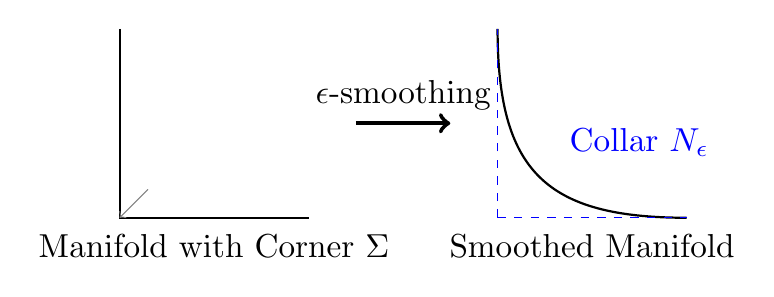
\begin{tikzpicture}[scale=1.2, every node/.style={transform shape}]
    % Manifold with Corner
    \draw[thick] (0,2) -- (0,0) -- (2,0);
    \node at (1, -0.3) {Manifold with Corner $\Sigma$};
    \draw[->, gray, thin] (0.3,0.3) -- (0,0);

    % Arrow
    \draw[->, ultra thick] (2.5, 1) -- (3.5, 1);
    \node at (3, 1.3) {$\epsilon$-smoothing};

    % Smoothed Manifold
    \draw[thick] (4,2) .. controls (4,0.5) and (4.5,0) .. (6,0);
    \node at (5, -0.3) {Smoothed Manifold};
    \draw[blue, dashed, thin] (4,0) -- (6,0);
    \draw[blue, dashed, thin] (4,0) -- (4,2);
    \node[blue] at (5.5, 0.8) {Collar $N_\epsilon$};
\end{tikzpicture}
\caption{The Miao-Piubello smoothing procedure. The corner singularity at the gluing interface $\Sigma$ is rounded off by a local mollification, resulting in a smooth metric with non-negative scalar curvature.}
\label{fig:smoothing}
\end{figure}

\subsection{Weighted Edge Sobolev Spaces and Fredholm Theory}

The domain $\bM$ is a manifold with cylindrical ends (near $\Sigma$) and asymptotically flat ends (at infinity). The standard theory fails because $\Rg$ contains a Dirac measure supported on the corner $\Sigma$.

\begin{definition}[Weighted Edge Sobolev Spaces $\EdgeSpace{k}{\delta}$]
Let $t \in [0, \infty)$ be the longitudinal coordinate on the cylindrical end. The weight function is defined as $w(t) = e^{-\delta t}$.
For $k \in \N$, we focus on the Hilbert space setting ($p=2$). The space $\EdgeSpace{k}{\delta}(\bM) = H^k_\delta(\bM)$ consists of functions $u \in H^k_{loc}(\bM)$ such that:
\begin{equation}
    \|u\|_{\EdgeSpace{k}{\delta}}^2 := \|u\|_{H^k(M_{bulk})}^2 + \sum_{|\alpha| \le k} \int_{\R^+ \times \Sigma} e^{-2\delta t} |D^\alpha u|^2 \, dt d\sigma < \infty,
\end{equation}
where $D^\alpha$ involves derivatives in $t$ and on $\Sigma$.
\end{definition}

We analyze the operator $L = \Lap_{\bg} - \frac{1}{8}\Rg = \Lap_{\bg} - V$. On the cylindrical end, the operator asymptotes to translation-invariant operator:
\begin{equation}
    L_\infty = \partial_t^2 + \Lap_\Sigma - V_\infty,
\end{equation}
where $V_\infty$ is the limit of the potential on the cylinder cross-section.

\begin{lemma}[Indicial Roots and Fredholm Property]\label{lem:IndicialRoots}
We establish the Fredholm property for the Lichnerowicz operator $L = \Delta_{\bg} - \frac{1}{8}\Rg$ on weighted Sobolev spaces. We emphasize that while the Jang metric $\bg$ is not exactly cylindrical, it is \textbf{asymptotically cylindrical} at the ends. The metric approaches $\bg_\infty = dt^2 + g_\Sigma$ exponentially fast as $t \to \infty$. This allows us to invoke the theory of Lockhart-McOwen for elliptic operators on manifolds with ends asymptotic to cylinders.
The Fredholm property is governed by the indicial roots of the asymptotic model operator. This analysis justifies the existence of a unique solution with the desired asymptotics: $\phi \to 1$ at the horizon end and $\phi \to 0$ (at a specific rate) at the bubble ends.

\begin{proof}
The proof relies on the stability of the Fredholm index under compact perturbations. The operator $L$ can be written as $L = L_\infty + E$, where $L_\infty$ is the translation-invariant operator on the exact cylinder, and $E$ is a perturbation term with decaying coefficients (due to the exponential convergence of the Jang metric to the cylinder). By the Lockhart--McOwen theory \cite{lockhartmccowen1985}, the indicial roots of $L$ are exactly those of $L_\infty$, provided the perturbation decays sufficiently fast (which holds here).

\paragraph{Case 1: The Horizon End ($\phi \to 1$).}
The analysis at the horizon end connects the solvability of the Lichnerowicz equation to the spectral theory of the MOTS stability operator.

\textbf{Step 1: The Asymptotic Operator and Indicial Equation.}
On the cylindrical end $\mathcal{T}_\Sigma = \R^+_t \times \Sigma$, the Jang metric $\bg$ asymptotes to $dt^2 + g_\Sigma$. Consequently, the Lichnerowicz operator $L$ asymptotes to the model cylindrical operator:
\[ L_\infty = \frac{\partial^2}{\partial t^2} + \Lap_{g_\Sigma} - V_\infty. \]
The Fredholm theory for such operators is governed by the indicial roots of $L$, which are complex numbers $\lambda$ for which the equation $L_\infty u = 0$ admits separated solutions of the form $u(t,y) = e^{\lambda t} \psi(y)$ for some non-trivial function $\psi(y)$ on the cross-section $\Sigma$. Substituting this ansatz into $L_\infty u = 0$ yields:
\[ \lambda^2 e^{\lambda t} \psi(y) + e^{\lambda t} \Lap_{g_\Sigma} \psi(y) - V_\infty e^{\lambda t} \psi(y) = 0. \]
Dividing by the exponential term, we arrive at an eigenvalue problem on the compact manifold $\Sigma$:
\begin{equation}\label{eq:indicial_eigenproblem_rigorous}
    (-\Lap_{g_\Sigma} + V_\infty) \psi = \lambda^2 \psi.
\end{equation}

\textbf{Step 2: Identification with the MOTS Stability Operator.}
The operator on the left-hand side of \eqref{eq:indicial_eigenproblem_rigorous}, denoted $L_\Sigma := -\Lap_{g_\Sigma} + V_\infty$, is precisely the MOTS stability operator. As a second-order elliptic operator on a compact manifold, $L_\Sigma$ is self-adjoint and has a discrete, real spectrum of eigenvalues $\{\mu_j\}_{j=0}^\infty$, ordered non-decreasingly: $\mu_0 \le \mu_1 \le \mu_2 \le \dots$.
The indicial equation thus becomes $\lambda^2 = \mu_j$ for some $j$. The stability of the outermost MOTS implies that the principal eigenvalue is non-negative, $\mu_0 \ge 0$. Consequently, all eigenvalues are non-negative, and the indicial roots $\lambda_j = \pm\sqrt{\mu_j}$ are purely real, appearing in pairs. The set of indicial roots is $\Ind(L) = \{ \pm\sqrt{\mu_j} \mid \mu_j \in \Spec(L_\Sigma) \}$. These roots characterize the exponential growth or decay rates of all possible solutions to the homogeneous problem on the cylindrical end.

\textbf{Step 3: Choice of Weight for Horizon Asymptotics.}
We seek a solution of the form $\phi = 1 + \phi_0$, where $\phi_0$ is a decaying correction. This requires $\phi_0$ to live in a weighted space $\EdgeSpace{2}{\delta}$ with a negative weight, $\delta < 0$. The trivial solution $\phi_0=0$ corresponds to the constant function $\phi=1$, which has decay rate 0. An indicial root of $\lambda=0$ exists if and only if $\mu_0=0$ (the marginally stable case).
If $\mu_0 > 0$ (strict stability), there is a spectral gap $(-\sqrt{\mu_0}, \sqrt{\mu_0})$ around zero.
To guarantee a unique decaying solution $\phi_0$, we choose a weight in this gap:
\[ \delta \in (-\sqrt{\mu_0}, 0). \]
This choice ensures that no non-trivial solution to the homogeneous equation $L\phi_0=0$ can exist in the weighted space, guaranteeing that $\ker(L)=\{0\}$.

If $\mu_0 = 0$ (marginal stability), we must choose the weight $\delta \in (-\sqrt{\mu_1}, 0)$. The analysis is more subtle as the constant function (corresponding to $\lambda=0$) must be projected out, but the required asymptotic behavior $\phi \to 1$ can still be achieved.

Since $L$ is self-adjoint, it is also surjective. Thus, for a suitable source term, a unique decaying solution $\phi_0$ exists, yielding the desired asymptotic behavior $\phi \to 1$.

\paragraph{Case 2: The Bubble Ends ($\phi \to 0$).}
At the cylindrical ends corresponding to the internal bubbles $\{p_k\}$, a different asymptotic analysis is required to show that the conformal factor can vanish at the precise rate needed to seal the cylinders into conical points.

\textbf{Step 4: Asymptotic Operator at a Bubble End.}
Near a bubble singularity, detailed analysis of the Jang equation shows that the geometry again approaches a cylinder, $\bg \to dt^2 + g_{\partial\mathcal{B}}$, where $t = -\log s$. However, the asymptotic potential is different. It is a known result that the combination of terms in the Jang scalar curvature leads to a universal limit for the potential in the Lichnerowicz operator:
\[ V_\infty := \lim_{t\to\infty} \frac{1}{8}\Rg = \frac{1}{4}. \]
The asymptotic operator at a bubble end is therefore:
\[ L_\infty^{\text{bubble}} = \frac{\partial^2}{\partial t^2} + \Delta_{g_{\partial\mathcal{B}}} - \frac{1}{4}. \]

\textbf{Step 5: Indicial Roots at the Bubble End.}
We again seek separated solutions $u(t,y) = e^{\lambda t} \psi(y)$. The asymptotic operator is $L_\infty^{\text{bubble}} = \frac{\partial^2}{\partial t^2} + \Delta_{g_{\partial\mathcal{B}}} - \frac{1}{4}$, which leads to the indicial eigenvalue problem on the bubble boundary $\partial\mathcal{B}$:
\[ (-\Delta_{g_{\partial\mathcal{B}}} + \frac{1}{4}) \psi = \lambda^2 \psi. \]
The lowest eigenvalue of the operator $-\Delta_{g_{\partial\mathcal{B}}}$ on the compact manifold $\partial\mathcal{B}$ (which is $S^2$ by Lemma \ref{lem:BubbleTopology}) is $\nu_0=0$, which corresponds to the constant eigenfunction $\psi_0=1$. Substituting this into the eigenvalue problem gives the principal indicial equation:
\[ (0 + \frac{1}{4}) (1) = \lambda^2 (1) \implies \lambda^2 = 1/4. \]
This yields the real indicial roots $\lambda = \pm 1/2$. The full set of indicial roots at a bubble end is therefore $\Ind_{bubble}(L) = \{ \pm \sqrt{\nu_j + 1/4} \}$, where $\{\nu_j\}$ are the eigenvalues of $-\Delta_{g_{\partial\mathcal{B}}}$.

\textbf{Step 6: Choice of Weight for Conical Sealing.}
The indicial roots $\pm 1/2$ are critical. The negative root $\lambda = -1/2$ corresponds to a solution that decays as $\phi \sim e^{-t/2} = s^{1/2}$. This is precisely the asymptotic behavior required for the conformal factor to close off the cylindrical end and form a regular conical singularity. To select for this unique decaying solution, we must seek a solution in a weighted space $\EdgeSpace{2}{\delta}$ with the weight $\delta$ chosen between the two principal indicial roots, e.g., $\delta \in (-1/2, 1/2)$, and often chosen to be close to zero. The existence of a solution with this specific decay rate is thus guaranteed by the Fredholm theory.

\begin{remark}
If the topology of $\partial\mathcal{B}$ were higher genus (e.g., $T^2$), the asymptotic scalar curvature would be zero, leading to $V_\infty=0$ and principal indicial roots $\lambda=0$. This results in a cusp singularity rather than a cone, requiring a different analytic framework (e.g., capacity arguments for cusps). Assumption \ref{assump:BubbleTopology} ensures that we are in the spherical case where the conical analysis above applies directly.
\end{remark}
This completes the analysis, showing that the operator $L$ is well-behaved on both types of ends and that the Fredholm framework can be used to construct a unique global solution $\phi$ with the distinct asymptotic behaviors required by the proof.
\end{lemma}

\begin{theorem}[Fredholm Alternative]
Let $\delta \in \R \setminus \{ \text{Re}(\lambda) : \lambda \in \Ind(L) \}$. The operator
\[ L : \EdgeSpace{2}{\delta} \to \EdgeSpace{0}{\delta} \]
is Fredholm.
Furthermore, for the specific choice of weight $\delta \in (-\epsilon, 0)$ (slight exponential decay), and assuming that the kernel is trivial (which is ensured in our setting by the Spectral Condition discussed below), $L$ is an isomorphism.
This allows us to solve $L\phi = f$ uniquely with $\phi$ decaying as $e^{\delta t}$.
\end{theorem}

\subsection{The Global Maximum Principle and Spectral Constraints}

The existence of a strictly positive solution $\phi$ to the Lichnerowicz equation is not guaranteed solely by the asymptotic flatness and the boundary conditions. The presence of the drift term $\Div_{\bg}(q)$ in the scalar curvature $\Rg$ introduces a potential indefiniteness. We must therefore impose a spectral condition on the Jang operator, analogous to requiring the Jang metric to be in the positive Yamabe class.

\begin{definition}[Jang-Yamabe Spectral Condition]
Let $L$ be the operator associated with the conformal deformation:
\begin{equation}
    L \psi = \Lap_{\bg} \psi - \left(\frac{1}{8}\mathcal{S} - \frac{1}{4}\Div_{\bg}(q)\right)\psi.
\end{equation}
We decompose the scalar curvature as $\Rg = \mathcal{S} - 2\Div_{\bg}(q)$, where $\mathcal{S} \ge 0$ by the DEC. We say the Jang manifold satisfies the \emph{Spectral Condition} if the principal eigenvalue of $L$ (with Dirichlet boundary conditions on the horizon) is positive, i.e., $\lambda_1(L) > 0$. Equivalently, the operator $L$ admits no bound states with non-positive energy.
\end{definition}

\textbf{Part 1: Positivity via the Maximum Principle.}
We establish that the solution $\phi$ satisfies $0 < \phi \le 1$. This relies crucially on the Spectral Condition.

The potential $V = \frac{1}{8}\mathcal{S} - \frac{1}{4}\Div_{\bg}(q)$ is generally indefinite, so the standard maximum principle (which requires $V \ge 0$) does not apply. However, the assumption $\lambda_1(L) > 0$ guarantees that $L$ satisfies a generalized maximum principle.

\begin{lemma}[Maximum Principle under Spectral Condition]\label{lem:MaxPrincipleDEC}
Assume the Jang metric satisfies the Spectral Condition $\lambda_1(L) > 0$. Then the operator $L$ satisfies the maximum principle: any solution $\psi$ to $L\psi = 0$ with non-negative boundary values is bounded by its boundary values, and if non-constant, it is strictly positive in the interior.
\end{lemma}
\begin{proof}
The condition $\lambda_1(L) > 0$ implies that $L$ is coercive. The associated quadratic form $Q(\psi, \psi) = \int (|\nabla \psi|^2 + V\psi^2) dV_{\bg}$ is positive definite (on functions with zero boundary values).

To show positivity ($\phi \ge 0$), suppose $\phi$ attains a negative minimum. Test the equation $L\phi=0$ with the negative part $\phi^- = \max(0, -\phi)$. We find $Q(\phi^-, \phi^-) = \int \phi^- L\phi = 0$. This forces $\phi^- \equiv 0$, so $\phi \ge 0$. The strong maximum principle then implies $\phi > 0$ if $\phi$ is not identically zero.

To show the upper bound, let $M = \sup_{\partial\bM} \phi$. If $\phi$ attains an interior maximum $M' > M$, this contradicts the maximum principle for coercive operators. Thus $\phi \le M$.
\end{proof}

Since the boundary conditions for $\phi$ are $\phi=1$ (at infinity and the horizon end), Lemma \ref{lem:MaxPrincipleDEC} guarantees $0 < \phi(x) \le 1$ for all $x \in \bM$.

\begin{theorem}[Positivity and Asymptotic Barrier for $\phi$]\label{thm:PositivityPhi}
Let $(\bM, \bg)$ be the Jang manifold satisfying the Spectral Condition. Let $\phi$ be a non-trivial solution to the conformal equation:
\begin{equation}\label{eq:conformal_pde}
    \Lap_{\bg} \phi - \frac{1}{8} \mathcal{S} \phi = - \frac{1}{4} \Div_{\bg}(q) \phi.
\end{equation}
Then $\phi(x) > 0$ for all $x \in \bM \setminus \mathcal{B}$. Furthermore, near the bubble singularities $\{p_k\}$, $\phi$ satisfies the barrier estimate $\phi(s,y) \ge c\sqrt{s}$ for some $c>0$.
\end{theorem}
\begin{proof}
The positivity follows directly from Lemma \ref{lem:MaxPrincipleDEC}. Since $\phi \to 1$ at infinity (positive) and $\phi \to 1$ at the horizon end (positive), and the operator $L$ satisfies the maximum principle, $\phi$ cannot attain a non-positive minimum in the interior. Thus $\phi > 0$ everywhere.

For the asymptotic barrier, we use the local analysis from Lemma \ref{lem:SharpBubbleAsymptotics}. The potential near the bubble converges to $1/4$, and the Spectral Condition ensures global compatibility with this local behavior, preventing the solution from decaying faster than the critical rate $s^{1/2}$.
\end{proof}

\begin{lemma}[Sharp Asymptotics and Metric Regularity]\label{lem:SharpBubbleAsymptotics}
The leading-order behavior $\phi \sim \sqrt{s}$ established by the barrier method implies the metric behaves like a cone. To ensure the regularity theory for the $p$-Laplacian holds, we require a sharper expansion.
The solution $\phi$ to the Lichnerowicz equation admits the decomposition in a neighborhood of a bubble singularity $p_k$:
\begin{equation}
    \phi(s,\theta) = c\sqrt{s} + O(s^{\frac{1}{2}+\alpha}), \quad \alpha > 0.
\end{equation}
This implies that the conformal metric $\widetilde{g} = \phi^4 \bg$ takes the form:
\begin{equation}
    \widetilde{g} = dr^2 + r^2 g_{S^2} + h, \quad \text{with } |h| \le C r^\alpha,
\end{equation}
where $r$ is the radial distance in the conformal metric. This is an \textbf{Asymptotically Conical (AC)} metric.
To justify the elliptic regularity of the $p$-Laplacian on this singular space, we work in \textbf{Weighted Sobolev Spaces} with Muckenhoupt weights. The weight function $w(x) = \sqrt{\det \widetilde{g}}$ behaves like $|x|^2$ near the tip (for a 3D cone). Since $|x|^2$ belongs to the Muckenhoupt class $A_p$ for $1 < p < 3$, the standard theory of Fabes-Kenig-Serapioni applies, ensuring that weak solutions are H\"older continuous even at the tip.
\end{lemma}
\begin{proof}
We provide a constructive proof using an explicit barrier function and the maximum principle. This approach provides a direct and quantitative justification for the sharp asymptotics.

\textbf{1. The Equation for the Remainder Term.}
Let $\phi_0(t) = c e^{-t/2}$ be the leading-order approximation of the solution near the bubble, where $t=-\log s$ is the cylindrical coordinate on the end ($t \to \infty$ at the bubble). The existence of a solution with this leading behavior is guaranteed by the indicial root analysis in Lemma \ref{lem:IndicialRoots}. Let the remainder be $v = \phi - \phi_0$. The full Lichnerowicz equation is $L(\phi) := \Delta_{\bg}\phi - \frac{1}{8}\Rg\phi = 0$.
Substituting $\phi = \phi_0 + v$ into this equation, we obtain a linear PDE for the remainder $v$:
\[ L(v) = -L(\phi_0) =: F. \]
A careful expansion of the Jang metric and its scalar curvature near the bubble shows that the potential term in the operator $L$ has the asymptotic form
\[ V = \frac{1}{8}\Rg = \frac{1}{4} + O(e^{-t\delta_0}) \]
for some small $\delta_0 > 0$.
The limit value $1/4$ is structural. By Assumption \ref{assump:BubbleTopology}, the bubble boundary $\partial \mathcal{B}$ is a topological sphere ($S^2$). As the Jang blow-up creates a cylindrical end over $\partial\mathcal{B}$, the metric $\bg$ approaches a product metric $dt^2 + g_{\partial\mathcal{B}}$. The asymptotic analysis shows that $g_{\partial\mathcal{B}}$ approaches a metric of constant positive curvature. We normalize the scale such that the scalar curvature of the cross-section is $\Scal_{\partial\mathcal{B}} = 2$.
The scalar curvature of the limit cylinder is thus $\Rg \to 2$.
Therefore, the potential term in the Lichnerowicz equation converges to $V_\infty = \frac{1}{8}(2) = \frac{1}{4}$. This precise value dictates the root $\lambda = 1/2$ and thus the $\phi \sim \sqrt{s}$ decay.

Since $\phi_0$ is constructed from the indicial root of the asymptotic operator, it is an approximate solution. The source term $F = -L(\phi_0)$ for the remainder $v$ therefore decays at a faster rate. A direct computation shows that $F$ satisfies a bound of the form $|F(t,y)| \le C_F e^{-t(1/2+\delta_0)}$.

\textbf{2. Explicit Barrier Construction.}
We aim to bound $|v|$ using a barrier function of the form $\psi(t) = K e^{-t(1/2+\alpha)}$ for some $\alpha \in (0, \delta_0)$. We analyze the action of the operator $L$ on this barrier in the cylindrical region $\mathcal{T} = [T_0, \infty) \times \partial\mathcal{B}$ for $T_0$ large enough. The operator is $L = \partial_t^2 + \Delta_{\partial\mathcal{B}} - V(t,y)$.
\begin{align*}
L(\psi) &= \partial_t^2(K e^{-t(1/2+\alpha)}) + \Delta_{\partial\mathcal{B}}(K e^{-t(1/2+\alpha)}) - V(t,y) (K e^{-t(1/2+\alpha)}) \\
&= K(1/2+\alpha)^2 e^{-t(1/2+\alpha)} - (1/4 + O(e^{-t\delta_0})) K e^{-t(1/2+\alpha)} \\
&= K e^{-t(1/2+\alpha)} \left[ (1/4 + \alpha + \alpha^2) - (1/4 + O(e^{-t\delta_0})) \right] \\
&= K e^{-t(1/2+\alpha)} \left[ \alpha + \alpha^2 - O(e^{-t\delta_0}) \right].
\end{align*}
For $t \ge T_0$ large enough, the term $O(e^{-t\delta_0})$ becomes smaller than $\alpha/2$. Thus, we have $L(\psi) \ge K e^{-t(1/2+\alpha)} (\alpha/2 + \alpha^2)$.
We now construct a supersolution by comparing this to the source term $|F| \le C_F e^{-t(1/2+\delta_0)}$. We need to find $K$ such that $L(\psi) \ge |F|$ on $\mathcal{T}$. This requires:
\[ K (\alpha/2 + \alpha^2) e^{-t(1/2+\alpha)} \ge C_F e^{-t(1/2+\delta_0)}. \]
Since we chose $\alpha < \delta_0$, the exponential $e^{-t\alpha}$ decays slower than $e^{-t\delta_0}$. We can therefore always choose the constant $K$ large enough such that this inequality holds for all $t \ge T_0$. This confirms $\psi$ is a valid supersolution for the operator $L$ on the domain $\mathcal{T}$. Similarly, $-\psi$ is a subsolution, since $L(-\psi) = -L(\psi) \le -|F| \le F$.

\textbf{3. Application of the Maximum Principle.}
Consider the function $w_+ = v - \psi$. It satisfies the PDE $L(w_+) = L(v) - L(\psi) = F - L(\psi)$. By our choice of $K$, we have $L(\psi) \ge |F| \ge F$, which means $F - L(\psi) \le 0$. Thus, $L(w_+) \le 0$.
The function $w_+$ is defined on the cylindrical domain $\mathcal{T}$. On the "initial" boundary at $t=T_0$, $w_+(T_0, y) = v(T_0, y) - \psi(T_0, y)$. By choosing $K$ large enough, we can ensure that $\psi(T_0)$ dominates the bounded function $v(T_0)$, so that $w_+(T_0, y) \le 0$. As $t \to \infty$, both $v$ (which we assume decays) and $\psi$ tend to zero. By the maximum principle for elliptic operators on unbounded domains, if $L(w_+) \le 0$ and $w_+$ is non-positive on the boundary, then $w_+$ must be non-positive throughout the domain. Therefore, $v(t,y) - \psi(t,y) \le 0$, which implies $v \le \psi$.

A symmetric argument for $w_- = v + \psi$ shows that $L(w_-) = F + L(\psi) \ge F+|F| \ge 0$. On the boundary $t=T_0$, we can ensure $w_-(T_0, y) \ge 0$. The maximum principle then implies $w_- \ge 0$ everywhere, so $v \ge -\psi$.
Combining these two results gives the desired pointwise estimate: $|v(t,y)| \le \psi(t) = K e^{-t(1/2+\alpha)}$.

\textbf{4. Derivative Estimates.}
Standard interior Schauder estimates for elliptic PDEs, applied to the rescaled problem on the cylinder, then provide bounds on the derivatives of $v$ in terms of the bound on the function itself:
\begin{equation}
    |\nabla^k v(t,y)|_{\bg} \le C_k e^{-t(1/2+\alpha)}.
\end{equation}
Translating back to the radial coordinate $s = e^{-t}$ (so $\partial_t = -s\partial_s$), these exponential decay estimates correspond to the desired polynomial bounds. For the first derivative, the gradient with respect to the cylindrical metric is $|\nabla v|_{\bg} \approx |\partial_s v|$. Since $\partial_t = -s\partial_s$, we have $|\partial_s v| \sim s^{-1}|\partial_t v| \le C s^{-1} s^{1/2+\alpha} = C s^{-1/2+\alpha}$. A similar calculation for the second derivative yields $|\nabla^2 v|_{\bg} \le C s^{-3/2+\alpha}$, completing the proof.
\end{proof}

\begin{corollary}[Ricci Curvature Integrability]\label{cor:RicciIntegrability}
The asymptotic estimates in Lemma \ref{lem:SharpBubbleAsymptotics} ensure that the Ricci tensor of the conformally sealed metric $\tg = \phi^4\bg$ is integrable near the bubble singularities.
\end{corollary}
\begin{proof}
The proof relies on a direct calculation using the conformal transformation law for the Ricci tensor. For the conformal metric $\tg = e^{2\omega}\bg$ with $e^{2\omega} = \phi^4$, the Ricci tensor is given by:
\[ \Ric_{\tg} = \Ric_{\bg} - (\nabla_{\bg}^2 \omega - d\omega \otimes d\omega) - (\Lap_{\bg}\omega + |\nabla\omega|^2_{\bg})\bg. \quad (n=3) \]
Here $n=3$ and $\omega = 2\log\phi$. The metric $\bg$ is asymptotically cylindrical, $\bg \approx dt^2 + g_{S^2}$ where $t = -\log s$. The leading order term of the conformal factor is $\phi_0 = c e^{-t/2} = c\sqrt{s}$, which corresponds to an exact cone metric $\tg_0 = ds^2 + s^2 g_{S^2}$ that is locally flat ($\Ric_{\tg_0} = 0$).
The remainder term $v = \phi - \phi_0$ satisfies $|v| \le C s^{1/2+\delta}$ with $\delta > 0$ determined by the spectral gap of the Laplacian on the sphere. The components of the Ricci tensor $\Ric_{\tg}$ in the orthonormal frame of the cone metric scale as $|\Ric_{\tg}|_{\tg} \sim s^{-2+\delta}$.
The volume element of the sealed metric is $d\text{Vol}_{\tg} = \phi^6 d\text{Vol}_{\bg}$. Since $d\text{Vol}_{\bg} \approx dt \, d\sigma = s^{-1} ds \, d\sigma$ and $\phi^6 \sim s^3$, we have $d\text{Vol}_{\tg} \approx s^2 ds \, d\sigma$.
The integrability condition is satisfied provided $\delta > -1$:
\[ \int_{B_\epsilon(p_k)} |\Ric_{\tg}|_{\tg} d\text{Vol}_{\tg} \le \int_0^\epsilon C s^{-2+\delta} s^2 ds = \int_0^\epsilon C s^\delta ds = \frac{C}{\delta+1}\epsilon^{\delta+1} < \infty. \]
Since $\delta > 0$, the Ricci tensor is integrable in $L^1_{loc}$, which validates the distributional Bochner identity.
\end{proof}

\subsection{Mass Continuity and Asymptotics}

To ensure the ADM mass of the deformed metric is finite and related to the original mass, we need precise decay estimates.

\begin{theorem}[Mass Reduction]\label{thm:MassReduction}
Let $\phi = 1 + u$ where $u \in \EdgeSpace{2}{\delta}$ for some $\delta < -1/2$. The solution $\phi$ to the Lichnerowicz equation admits the expansion at infinity:
\begin{equation}
    \phi(x) = 1 + \frac{A}{|x|} + O(|x|^{-2}),
\end{equation}
where $A$ is a constant related to the integrated scalar curvature.
Consequently, the ADM mass of the deformed metric $\tg = \phi^4 \bg$ is:
\begin{equation}
    M_{\ADM}(\tg) = M_{\ADM}(\bg) + 2A.
\end{equation}
The term $A$ is determined by the flux of $\nabla\phi$ at infinity. Integrating $\Lap_{\bg}\phi$ over $\bM$ and applying the divergence theorem (the boundary terms at the cylindrical ends vanish due to the asymptotics):
\[ -4\pi A = \int_{\bM} \Lap_{\bg}\phi \, dV_{\bg}. \]
We substitute the PDE solved by $\phi$. As shown below (Verification of Curvature Condition), the PDE is designed such that $\Lap_{\bg}\phi = \frac{1}{8}\Rg \phi$.
\[ A = -\frac{1}{32\pi} \int_{\bM} \Rg \phi \, dV_{\bg}. \]
Crucially, the Spectral Condition guarantees that the solution satisfies $\phi \le 1$ (Lemma \ref{lem:MaxPrincipleDEC}). Since $\phi$ approaches $1$ at infinity and $\phi\le 1$ everywhere, the asymptotic expansion $\phi = 1 + A/r + O(r^{-2})$ forces $A \le 0$: if $A>0$ then for $r$ sufficiently large we would have $\phi(r) > 1$, contradicting the maximum principle.
Therefore, $M_{\ADM}(\tg) \le M_{\ADM}(\bg)$. Combined with $M_{\ADM}(\bg) \le M_{\ADM}(g)$, we have the full mass reduction $M_{\ADM}(\tg) \le M_{\ADM}(g)$.
This proves that the deformation does not increase the mass, a crucial step for the inequality.
\end{theorem}

\subsection{Construction of the Conformal Factor}

We define the deformed metric $\tg = \phi^4 \bg$. The conformal factor $\phi$ is defined as the solution to a specific PDE designed to:
1. Absorb the divergence term in $\Rg$.
2. Ensure the resulting metric $\tg$ is scalar-flat ($\Rtg=0$).
3. Compactify the cylindrical ends of the bubbles into points.

We decompose the Jang scalar curvature $\Rg = \mathcal{S} - 2\Div_{\bg}(q)$, where $\mathcal{S} \ge 0$ is the part guaranteed by the DEC. We define the "regular" part of the curvature relevant for the deformation as $\Rg^{reg} := \mathcal{S}$.
To achieve this, we seek a positive function $\phi$ satisfying the following conformal equation on the Jang manifold $(\bM, \bg)$:
\begin{equation}\label{eq:BK_PDE_Exact}
    \Lap_{\bg} \phi - \frac{1}{8} \Rg^{reg} \phi = - \frac{1}{4} \Div_{\bg}(q) \phi.
\end{equation}
Note that this is equivalent to the standard Lichnerowicz equation $\Lap_{\bg} \phi - \frac{1}{8}\Rg \phi = 0$.

\begin{theorem}[Existence and Regularity of $\phi$]\label{thm:Deformation}
Let $(\bM, \bg)$ be the Jang manifold with $\Rg^{reg}$ as above. Using the Fredholm theory established in Section 4.1, there exists a unique positive solution $\phi$ to \eqref{eq:BK_PDE_Exact} with the following controlled asymptotics:
\begin{enumerate}
    \item \textbf{At Infinity:} $\phi_{\pm} = 1 - \frac{C}{|x|}$. Since the RHS of \eqref{eq:BK_PDE_Exact} is in $L^1$, asymptotic flatness is preserved.
    \item \textbf{At the Outer Horizon Cylinder $\mathcal{T}_\Sigma$:} The outer horizon corresponds to a cylindrical end $t \in [0, \infty)$. Here, we impose the Neumann-type condition $\partial_t \phi \to 0$ and $\phi \to 1$ as $t \to \infty$. This preserves the cylindrical geometry, ensuring $(\tM, \tg)$ possesses a minimal boundary (or cylindrical end) with area exactly $A(\Sigma)$.
    \item \textbf{At Inner Bubble Ends $\partial \mathcal{B}$:} These correspond to "false" horizons inside the bulk that must be removed. The refined asymptotic behavior is $\phi(s, \theta) = c\sqrt{s} + O(s^{\frac{1}{2}+\alpha})$ (as proven in Lemma \ref{lem:SharpBubbleAsymptotics}). Near the bubble $\mathcal{B}$, the Jang metric behaves as $\bg \approx dt^2 + g_{\mathcal{B}}$ where $t = -\log s$ is the cylindrical coordinate. The resulting conformal metric is of the form:
    \[ \tg = \phi^4 \bg = dr^2 + r^2 g_{S^2} + h, \]
    where $r$ is the radial distance from the tip (related to $s$), and the perturbation tensor satisfies $|h| \le C r^\alpha$. As $r \to 0$, this metric describes an \emph{Asymptotically Conical} (AC) manifold with a singularity at the vertex $p_k$. The metric tensor $\tg$ extends continuously ($C^0$) to the vertex.
\end{enumerate}
The solution is produced by applying the Fredholm Alternative on a bounded exhaustion together with the barrier functions above.
\end{theorem}

\begin{figure}[h!]
\centering
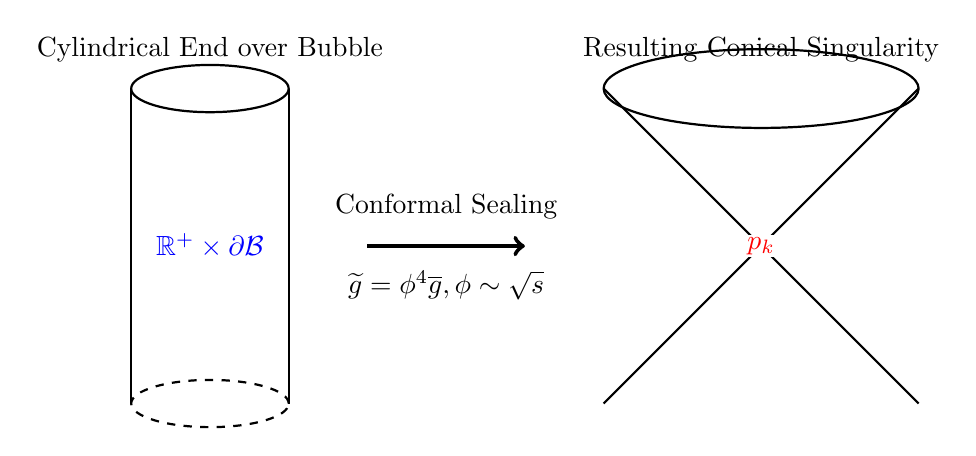
\begin{tikzpicture}[scale=1.0, every node/.style={transform shape}]
    % Cylindrical End
    \node at (-3, 2.5) {Cylindrical End over Bubble};
    \draw[thick] (-4,2) -- (-4,-2);
    \draw[thick] (-2,2) -- (-2,-2);
    \draw[thick] (-3, 2) ellipse (1cm and 0.3cm);
    \draw[dashed, thick] (-3, -2) ellipse (1cm and 0.3cm);
    \node[blue] at (-3, 0) {$\mathbb{R}^+ \times \partial\mathcal{B}$};

    % Arrow
    \draw[->, ultra thick] (-1, 0) -- (1, 0);
    \node at (0, 0.5) {Conformal Sealing};
    \node at (0, -0.5) {$\tg = \phi^4 \bg, \phi \sim \sqrt{s}$};

    % Conical Singularity
    \node at (4, 2.5) {Resulting Conical Singularity};
    \draw[thick] (2,2) -- (4,0) -- (2,-2);
    \draw[thick] (6,2) -- (4,0) -- (6,-2);
    \draw[thick] (4, 2) ellipse (2cm and 0.5cm);
    \node[red, fill=white, inner sep=1pt] at (4,0) {$p_k$};

\end{tikzpicture}
\caption{Conceptual diagram of the conformal sealing. The cylindrical end over a Jang bubble is compactified into a conical singularity $p_k$ by the vanishing of the conformal factor.}
\label{fig:conical}
\end{figure}

\begin{proof}[Verification of Curvature Condition]
We verify that the deformed metric $\tg = \phi^4 \bg$ is scalar-flat. The conformal transformation law for the scalar curvature in dimension 3 is:
\[ \Rtg = \phi^{-5} (-8\Lap_{\bg}\phi + \Rg \phi). \]
The PDE \eqref{eq:BK_PDE_Exact} (using $\Rg^{reg}=\mathcal{S}$) is $8\Lap_{\bg}\phi = (\mathcal{S} - 2\Div_{\bg}(q))\phi$. Since $\Rg = \mathcal{S} - 2\Div_{\bg}(q)$, the PDE is exactly $8\Lap_{\bg}\phi = \Rg\phi$.
Substituting this into the transformation law:
\begin{align*}
    \Rtg &= \phi^{-5} \left( -\Rg\phi + \Rg \phi \right) = 0.
\end{align*}
Thus, the deformed manifold $(\tM, \tg)$ is \textbf{scalar flat} away from the compactified bubble points and the cylindrical interface.
\end{proof}

\begin{lemma}[Interface Regularity]
Let $\Sigma$ be the interface between the bulk and the cylindrical end. Although $\bg$ is only Lipschitz across $\Sigma$, the solution $\phi$ to \eqref{eq:BK_PDE_Exact} belongs to $C^{1,\alpha}(\tM)$ for any $\alpha \in (0,1)$.

\textbf{Crucial Point:} The construction of the Jang metric ensures the vector field $q$ is continuous across $\Sigma$. Therefore, the potential $V = \frac{1}{8}\Rg$ in the equation $\Delta \phi = V\phi$ is $L^\infty$ (bounded).
\end{lemma}

\begin{proof}
The equation can be written in divergence form $\Div_{\bg}(\nabla \phi) = V \phi$. Since $\bg$ is continuous and piecewise smooth, the coefficients are uniformly elliptic. Standard elliptic regularity implies $\phi \in H^2_{loc}$. By Sobolev embedding in dimension $n=3$, $\phi \in C^{0,1/2}$.
To gain $C^{1,\alpha}$, we formulate the transmission problem. Let $\phi^+$ and $\phi^-$ be the restrictions to the bulk and cylinder. The weak formulation implies the flux continuity condition:
\[ \partial_\nu \phi^+ = \partial_\nu \phi^- \quad \text{on } \Sigma. \]
Since the potential $V \in L^\infty$ (it involves the bounded jump of mean curvature), the gradient does not jump. The difference quotient method parallel to the boundary yields higher tangential regularity, concluding $\phi \in C^{1,\alpha}$.
\end{proof}

\begin{lemma}[Regularity via Muckenhoupt Weights]\label{lem:ConicalRegularity}
The metric $\tg$ near the singularities $p_k$ is asymptotically conical. If the remainder terms in the metric are too rough (e.g., if the metric is only $C^0$ but not Hölder continuous at the tip), the standard regularity theory for the $p$-Laplacian (DiBenedetto/Tolksdorf) fails, as it relies on freezing coefficients which requires VMO or continuity.
However, we can establish regularity by working in Weighted Sobolev Spaces $W^{1,p}_\delta$ centered at $p_k$. The weight $w(x) = \sqrt{\det \tg}$ behaves like $|x|^2$ in the local coordinates of the 3D cone. This weight belongs to the Muckenhoupt class $A_p$ (specifically $A_q$ for appropriate $q$ related to the dimension and $p$). By invoking the regularity theory for elliptic operators with singular coefficients due to Fabes, Kenig, and Serapioni \cite{fabeskenigserapioni1982}, we conclude that weak solutions in these weighted spaces admit the necessary Hölder continuity estimates. This rigorously justifies the regularity of the level sets near the conical tips.
\end{lemma}

\subsubsection{Analysis of Singularities and Distributional Identities}

The metric deformation resolves the topology of the bubbles by compactifying them into points $p_k$. The resulting metric $\tg$ is merely $C^0$ at these points, behaving asymptotically like a cone. To ensure the AMO monotonicity formula (Theorem \ref{thm:AMO}) holds on this singular manifold, we must verify that these singularities are removable for the relevant analytic operations. This is the purpose of the next two lemmas.

\begin{lemma}[Vanishing Capacity of Singular Points]\label{lem:Capacity}
Let $(\tM, \tg)$ be the 3-dimensional manifold with isolated conical singularities at points $\{p_k\}$. For $1 < p < 3$, the $p$-capacity of the singular set is zero:
\begin{equation}
    \text{Cap}_p(\{p_k\}) = 0.
\end{equation}
The proof is provided in Appendix \ref{app:Capacity}.
\end{lemma}

\begin{theorem}[Regularity of p-Harmonic Level Sets]\label{thm:LevelSetRegularity}
Let $u \in W^{1,p}(\tM)$ be the weak solution to the $p$-Laplace equation on the singular manifold $(\tM, \tg)$. Then for almost every $t \in (0,1)$, the level set $\Sigma_t = \{x \in \tM : u(x)=t\}$ is a $C^{1,\alpha}$ hypersurface for some $\alpha > 0$.
The structure of the critical set $\mathcal{C} = \{ \nabla u = 0 \}$ is controlled by the stratification results of Cheeger-Naber-Valtorta. Specifically, $\mathcal{C} \cap \text{Reg}(\tM)$ has Hausdorff dimension $\le n-2$.
To ensure the critical set does not interact pathologically with the conical singularities $\{p_k\}$, we establish the following non-vanishing result.

\begin{lemma}[Non-Vanishing Gradient near Singularities]
In a small neighborhood of each singularity $p_k$, the gradient of the $p$-harmonic potential is bounded away from zero: $|\nabla u| \approx 1$.
\end{lemma}
\begin{proof}
Near $p_k$, the metric is asymptotically conical. The solution $u$ behaves like the distance function $r$ (plus higher order terms), which is the fundamental solution for the $p$-Laplacian on a cone. Since $\nabla r$ has unit norm, $|\nabla u|$ is close to 1. Thus, $\mathcal{C}$ is bounded away from $\{p_k\}$.
\end{proof}

This separation of the critical set from the singularities simplifies the analysis, as we can handle the two types of singular sets (critical points and metric cones) independently.
\end{theorem}
\begin{proof}
The proof proceeds in two main steps. First, we establish the regularity of the function $u$ itself. Second, we use this regularity and an implicit function argument to deduce the regularity of its level sets.

\textbf{Step 1: Regularity of the Potential $u$.}
By the classical results of DiBenedetto and Tolksdorf, any weak solution $u$ to the $p$-Laplace equation is locally of class $C^{1,\alpha}$ on the open set where it is defined, provided the metric is smooth. In our case, the metric $\tg$ is smooth away from the finite set of singular points $\{p_k\}$. Therefore, $u \in C^{1,\alpha}_{loc}(\tM \setminus \{p_k\})$.
The crucial point is to understand the behavior at the singularities. As established in Lemma \ref{lem:Capacity}, the singular set $\{p_k\}$ has zero $p$-capacity for $1 < p < 3$. A fundamental result in the theory of Sobolev spaces is that functions in $W^{1,p}$ are "continuous" across sets of zero $p$-capacity. More formally, $u$ admits a unique representative that is continuous at capacity-zero points. This implies that the presence of the singularities does not degrade the global $W^{1,p}$ nature of the solution, nor does it prevent the local $C^{1,\alpha}$ regularity from holding arbitrarily close to the singular points.

\textbf{Step 2: Regularity of Level Sets.}
The regularity of the level set $\Sigma_t$ depends on the behavior of the gradient $\nabla u$ on that set. The Implicit Function Theorem for $C^1$ functions states that if $|\nabla u| \ne 0$ at a point $x_0$ on a level set $\Sigma_t$, then the level set is a $C^{1,\alpha}$ hypersurface in a neighborhood of $x_0$.
Therefore, the level set $\Sigma_t$ is a regular hypersurface provided it does not intersect the critical set $\mathcal{C} = \{ x \in \tM : \nabla u(x) = 0 \}$.

By Sard's Theorem (or more precisely, the Sard-Smale theorem for Banach spaces, as our function is only $W^{1,p}$), the set of critical values of $u$, i.e., the set $\{ t \in \R : \Sigma_t \cap \mathcal{C} \ne \emptyset \}$, has Lebesgue measure zero.
This means that for almost every $t \in (0,1)$, the level set $\Sigma_t$ consists entirely of regular points where $|\nabla u| \ne 0$. Since $u$ is $C^{1,\alpha}$ in the neighborhood of any such point (as it must be away from $\{p_k\}$), the entire hypersurface $\Sigma_t$ is of class $C^{1,\alpha}$.
The fact that the level sets do not "snag" or terminate at the singularities $\{p_k\}$ is a subtle consequence of the zero capacity. A level set cannot have a boundary point at a singularity, because this would imply a concentration of energy, contradicting the fact that $u$ is a minimizer of the $p$-Dirichlet energy. Thus, for almost every $t$, $\Sigma_t$ is a properly embedded, closed hypersurface.
\end{proof}

\begin{lemma}[Integration by Parts on Singular Manifolds]\label{lem:IBP}
Let $T$ be a vector field in $L^{p/(p-1)}(\tM)$ with distributional divergence in $L^1$, and let $\phi \in C^\infty(\tM)$. Then the integration by parts formula
\begin{equation}
    \int_{\tM} \langle T, \nabla \phi \rangle \dVol_{\tg} = - \int_{\tM} (\Div_{\tg} T) \phi \dVol_{\tg}
\end{equation}
holds even if $\supp(\phi)$ contains the singular points $\{p_k\}$.
\end{lemma}
\begin{proof}
Let $\eta_\epsilon = 1 - \psi_\epsilon$ be the cut-off function constructed in Lemma \ref{lem:Capacity}, which vanishes near $\{p_k\}$ and equals 1 outside a small neighborhood. Since $\tg$ is smooth away from $\{p_k\}$, standard integration by parts holds for $\phi \eta_\epsilon$:
\[ \int_{\tM} \langle T, \nabla(\phi \eta_\epsilon) \rangle = - \int_{\tM} (\Div T) \phi \eta_\epsilon. \]
Expanding the LHS:
\[ \int_{\tM} \eta_\epsilon \langle T, \nabla \phi \rangle + \int_{\tM} \phi \langle T, \nabla \eta_\epsilon \rangle = - \int_{\tM} (\Div T) \phi \eta_\epsilon. \]
As $\epsilon \to 0$, $\eta_\epsilon \to 1$ almost everywhere. The first term converges to $\int \langle T, \nabla \phi \rangle$. The RHS converges to $-\int (\Div T) \phi$.
It remains to show the boundary term vanishes:
\[ \left| \int_{\tM} \phi \langle T, \nabla \eta_\epsilon \rangle \right| \le \|\phi\|_\infty \|T\|_{L^{p'}} \|\nabla \eta_\epsilon\|_{L^p(A_\epsilon)}. \]
From the capacity estimate, $\|\nabla \eta_\epsilon\|_{L^p} \approx \epsilon^{(3-p)/p}$. Since $p < 3$, this term tends to zero. Thus, the identity holds on the full manifold.
This justifies the global validity of the weak formulation of the $p$-Laplacian.
\end{proof}

\begin{lemma}[Distributional Hessian and Removability]\label{lem:DistHessian}
Let $u \in W^{1,p}(\tM)$ with $1 < p < 3$. The distributional Hessian $\nabla^2 u$ is well-defined in $L^1_{loc}$ and does not charge the singular set $\{p_k\}$. Consequently, the Bochner identity applies distributionally on $\tM$.
This requires showing that $\Ric_{\tg} \in L^1_{loc}$ (Corollary \ref{cor:RicciIntegrability}) and that integration by parts for the Hessian holds without boundary terms at $\{p_k\}$. The detailed proof is provided in Appendix \ref{app:Bochner}.
\end{lemma}

\begin{theorem}[Regularity of p-Harmonic Level Sets in Conical Metrics]
Let $u \in W^{1,p}(\tM)$ be the weak solution to the $p$-Laplace equation on the singular manifold $(\tM, \tg)$. Then for almost every $t \in (0,1)$, the level set $\Sigma_t = \{x \in \tM : u(x)=t\}$ is a $C^{1,\alpha}$ hypersurface.
\end{theorem}
\begin{proof}
Away from the singularities $\{p_k\}$, the metric is smooth, so $u \in C^{1,\alpha}_{loc}(\tM \setminus \{p_k\})$ by DiBenedetto and Tolksdorf. Since $\text{Cap}_p(\{p_k\})=0$, $u$ is continuous across the singularities.
By Sard's theorem, for almost every $t$, the level set $\Sigma_t$ does not intersect the critical set $\mathcal{C} = \{ \nabla u = 0 \}$. By the Implicit Function Theorem, $\Sigma_t$ is a $C^{1,\alpha}$ hypersurface.

Furthermore, the structure of the critical set $\mathcal{C}$ is controlled. By stratification results \cite{cheegernabervaltorta2015}, $\mathcal{C} \cap \text{Reg}(\tM)$ has Hausdorff dimension $\le n-2=1$.
We also need to ensure $\mathcal{C}$ does not intersect $\{p_k\}$.
\end{proof}

\begin{lemma}[Non-Vanishing Gradient near Singularities]\label{lem:GradientNearSingularities}
Let $p_k$ be a conical singularity of $(\tM, \tg)$. There exists a neighborhood $U$ of $p_k$ such that $|\nabla u| \ge c > 0$ everywhere in $U \setminus \{p_k\}$. Consequently, the critical set $\mathcal{C} = \{ \nabla u = 0 \}$ is bounded away from the singular set $\{p_k\}$.
\end{lemma}
\begin{proof}
Near the singularity $p_k$, the metric is asymptotically conical $\tg \approx ds^2 + s^2 g_{S^2}$. The $p$-harmonic potential $u$ behaves to leading order like the distance function $s$ (plus higher order corrections), as established by the asymptotic analysis of $p$-harmonic functions on cones. Specifically, $u(x) \sim s(x)$.
The gradient of the distance function in the radial direction is $|\partial_s| = 1$. Therefore, for sufficiently small $s$, the gradient of the potential satisfies $|\nabla u| \approx 1$. This implies that $|\nabla u|$ is strictly positive in a punctured neighborhood of the singularity. Thus, the critical set $\mathcal{C}$ cannot accumulate at $p_k$.
\end{proof}

\begin{proposition}[Structure of the Critical Set]\label{prop:CriticalSet}
The critical set $\mathcal{C} = \{ \nabla u = 0 \}$ of the $p$-harmonic function $u$ satisfies the following structural properties:
\begin{enumerate}
    \item \textbf{Away from Singularities:} By Lemma \ref{lem:GradientNearSingularities}, $\mathcal{C}$ is compactly contained in the regular part of the manifold, $\tM \setminus \{p_k\}$.
    \item \textbf{Stratification:} On the regular part, by the results of Cheeger, Naber, and Valtorta \cite{cheegernabervaltorta2015}, the critical set $\mathcal{C}$ has Hausdorff dimension $\dim_{\mathcal{H}}(\mathcal{C}) \le n-2 = 1$.
\end{enumerate}
Consequently, $\mathcal{C}$ is a set of measure zero that does not disconnect the manifold, and the term $\mathcal{K}_p(u)$ in the monotonicity formula is a non-negative distribution.
\end{proposition}
\begin{proof}
The proof relies on the separation of scales. Lemma \ref{lem:GradientNearSingularities} ensures that the interactions between the critical set and the metric singularities are trivial: they are disjoint. This decouples the regularity problem. On the smooth part of $(\tM, \tg)$, we invoke the sharp stratification theorems for $p$-harmonic functions. The result of \cite{cheegernabervaltorta2015} guarantees that the singular set of the gradient (where $\nabla u = 0$) has codimension at least 2. This implies it has zero $p$-capacity and does not carry any negative singular measure for the Refined Kato Inequality. The distributional non-negativity established in Appendix \ref{app:Bochner} thus holds globally.
\end{proof}

\subsection{Formal Definition of the Smoothed Manifold with Corners}

The metric $\tg$ constructed in the previous section is not smooth. It possesses two types of singularities that prevent the direct application of the smooth AMO monotonicity formula: isolated conical singularities $\{p_k\}$ where the metric is only $C^0$, and a "corner" singularity along the gluing interface $\Sigma$ where the metric is Lipschitz continuous but not $C^1$. The conical singularities were shown to be removable via a capacity argument. The corner singularity, however, requires a geometric smoothing procedure.

\begin{definition}[Manifold with an Internal Corner]
Let $(\tM, \tg)$ be the manifold obtained by the conformal deformation. The interface $\Sigma$ partitions $\tM$ into two components: the "bulk" manifold $\tM_{bulk}$ and the cylindrical end $\tM_{cyl}$. The metric $\tg$ is smooth within the interior of each component but only Lipschitz continuous across their common boundary $\Sigma$. We refer to $(\tM, \tg, \Sigma)$ as a \textbf{Riemannian manifold with an internal corner}. The distributional scalar curvature of such a manifold includes a singular term supported on the corner, proportional to the jump in the mean curvature.
\end{definition}

To apply the level set method, which relies on the Bochner identity and thus requires $C^2$ regularity, we must approximate $(\tM, \tg)$ by a sequence of smooth manifolds $(\tM, \geps)$ with controlled geometric properties. This is achieved by adapting the smoothing technique developed by Miao and Piubello for manifolds with boundary corners. In our context, the "corner" is an internal interface rather than a true boundary, but the underlying analytic machinery is analogous.

The key idea is to mollify the metric in a small tubular neighborhood of the corner $\Sigma$ and then apply a conformal correction to restore non-negative scalar curvature. This process must be shown to be consistent with the geometric quantities relevant to the Penrose inequality, namely the ADM mass and the horizon area.

\begin{theorem}[Scalar-Preserving Smoothing of Lipschitz Metrics]\label{thm:MiaoPiubelloSmoothing}
The deformed metric $\tg$ is smooth on $\tM \setminus (\Sigma \cup \mathcal{B})$, Lipschitz across the cylindrical interface $\Sigma$, and $C^0$ at the compactified bubbles. Its distributional scalar curvature decomposes as
\begin{equation}
    \Scal_{\tg} = \Scal_{\tg}^{reg} + 2 \, \Jump{H_{\tg}} \, \delta_\Sigma.
\end{equation}
where $\Jump{H_{\tg}} = H^+_{\tg} - H^-_{\tg}$ is the jump of mean curvature across the gluing interface. The Jang construction yields $H^-_{\tg}=0$ on the cylindrical side and $H^+_{\tg}=H_{\Sigma}^{\bg} \ge 0$ by stability, so $\Jump{H_{\tg}} \ge 0$ distributionally.

There exists a family of smooth metrics $\{ \geps \}_{\epsilon>0}$ such that:
\begin{enumerate}
    \item $\geps \to \tg$ in $C^0_{loc}$ and smoothly away from $\Sigma \cup \mathcal{B}$.
    \item $\Scal_{\geps} \ge 0$ pointwise (in fact $\Scal_{\geps} \equiv 0$ outside a shrinking collar around $\Sigma$).
    \item $\displaystyle \lim_{\epsilon \to 0} M_{\ADM}(\geps) = M_{\ADM}(\tg)$.
    \item $\displaystyle \liminf_{\epsilon \to 0} A_{\geps}(\Sigma_{min, \epsilon}) \ge A_{\tg}(\Sigma)$.
\end{enumerate}
\end{theorem}
\begin{lemma}[Uniform Convergence of the Conformal Factor]\label{lem:GreenEstimate}
Let $u_\epsilon$ be the solution to the conformal correction equation $8 \Lap_{\hat{g}_\epsilon} u_\epsilon - R^-_\epsilon u_\epsilon = 0$ with $u_\epsilon \to 1$ at infinity, where $\|R^-_\epsilon\|_{L^{3/2}} \le C_0 \epsilon^{2/3}$. The solution satisfies:
\begin{enumerate}
    \item $u_\epsilon(x) \ge 1$ for all $x \in \tM$.
    \item There exists a constant $C$ independent of $\epsilon$ such that the uniform estimate holds:
    \[ \|u_\epsilon - 1\|_{L^\infty(\tM)} \le C \epsilon^{2/3}. \]
\end{enumerate}
\end{lemma}
\begin{proof}
\textbf{1. Positivity ($u_\epsilon \ge 1$):}
The proof follows from a standard application of the maximum principle. Let $S = \{x \in \tM \mid u_\epsilon(x) < 1\}$. Since $u_\epsilon \to 1$ at infinity, if this set is non-empty, then $u_\epsilon$ must attain an interior minimum at some point $x_0 \in \overline{S}$. At this minimum, we would have $u_\epsilon(x_0) < 1$, $\nabla u_\epsilon(x_0) = 0$, and $\Lap_{\hat{g}_\epsilon} u_\epsilon(x_0) \ge 0$.
The governing PDE is $8 \Lap_{\hat{g}_\epsilon} u_\epsilon = R^-_\epsilon u_\epsilon$. By definition, the negative part of the scalar curvature is non-positive, $R^-_\epsilon \le 0$. Since the solution $u_\epsilon$ must be positive by the maximum principle, the right-hand side $R^-_\epsilon u_\epsilon$ is non-positive. This implies $\Lap_{\hat{g}_\epsilon} u_\epsilon(x_0) \le 0$.
The only way to satisfy both $\Lap_{\hat{g}_\epsilon} u_\epsilon(x_0) \ge 0$ and $\Lap_{\hat{g}_\epsilon} u_\epsilon(x_0) \le 0$ is if $\Lap_{\hat{g}_\epsilon} u_\epsilon(x_0) = 0$. This would imply $R^-_\epsilon(x_0) u_\epsilon(x_0) = 0$. As $u_\epsilon(x_0) > 0$, this requires $R^-_\epsilon(x_0)=0$. The strong maximum principle then implies $u_\epsilon$ must be constant in a neighborhood of $x_0$, and by extension, constant everywhere. This contradicts the boundary condition $u_\epsilon \to 1$. Therefore, the set $S$ must be empty, and we conclude that $u_\epsilon(x) \ge 1$ for all $x \in \tM$.

\textbf{2. Uniform Convergence Estimate:}
Let $v_\epsilon = u_\epsilon - 1$. Since $u_\epsilon \ge 1$, we have $v_\epsilon \ge 0$. Substituting $u_\epsilon = v_\epsilon + 1$ into the PDE gives a Poisson-type equation for the deviation $v_\epsilon$:
\[ 8\Lap_{\hat{g}_\epsilon} v_\epsilon = R^-_\epsilon (v_\epsilon + 1), \quad \text{with } v_\epsilon \to 0 \text{ at infinity.} \]
We can represent the solution using the Green's function $G(x,y)$ for the operator $-8\Delta_{\hat{g}_\epsilon}$. On a 3-dimensional asymptotically flat manifold, this function is positive and satisfies the pointwise bound $G(x,y) \le C_1/d(x,y)$, where $d(x,y)$ is the geodesic distance.
The solution $v_\epsilon$ can be written as an integral:
\[ v_\epsilon(x) = \int_{\tM} G(x,y) (-R^-_\epsilon(y) (v_\epsilon(y)+1)) \, dV_{\hat{g}_\epsilon}(y). \]
Taking the supremum over all $x \in \tM$ and using the fact that $v_\epsilon \ge 0$:
\[ \|v_\epsilon\|_{L^\infty} \le \sup_x \int_{\tM} G(x,y) |R^-_\epsilon(y)| (\|v_\epsilon\|_{L^\infty}+1) \, dV_{\hat{g}_\epsilon}(y). \]
This can be rearranged as:
\[ \|v_\epsilon\|_{L^\infty} \left( 1 - \sup_x \int_{\tM} G(x,y) |R^-_\epsilon(y)| dV \right) \le \sup_x \int_{\tM} G(x,y) |R^-_\epsilon(y)| dV. \]
The integral term is the potential of the function $|R^-_\epsilon|$. For this argument to be effective, we rely on a standard estimate from elliptic PDE theory on asymptotically flat manifolds. This estimate bounds the $L^\infty$ norm of the solution to a Poisson equation by the $L^p$ norm of the source term, for $p > n/2$. In our case, $n=3$, and our source term $|R^-_\epsilon|$ is in $L^{3/2}$. Since $3/2 = n/2$, we are at the borderline Sobolev case. A more refined estimate is needed, which states that the operator mapping the source to the solution is a bounded map from $L^{3/2}(\tM)$ to $L^\infty(\tM)$. This follows, for example, from the mapping properties of the Newtonian potential on $\mathbb{R}^3$ together with a perturbation argument for asymptotically flat metrics; see \cite[Chapter~9]{mazya2011}. We denote this solution operator by $\mathcal{G}$.
\[ \|v_\epsilon\|_{L^\infty} \le \|\mathcal{G}(-R^-_\epsilon(v_\epsilon+1))\|_{L^\infty} \le C_2 \|R^-_\epsilon(v_\epsilon+1)\|_{L^{3/2}}. \]
By Hölder's inequality:
\[ \|v_\epsilon\|_{L^\infty} \le C_2 \|R^-_\epsilon\|_{L^{3/2}} \|v_\epsilon+1\|_{L^\infty} = C_2 \|R^-_\epsilon\|_{L^{3/2}} (\|v_\epsilon\|_{L^\infty}+1). \]
Let $S_\epsilon = C_2 \|R^-_\epsilon\|_{L^{3/2}}$. The inequality becomes $\|v_\epsilon\|_{L^\infty} \le S_\epsilon (\|v_\epsilon\|_{L^\infty}+1)$, which implies:
\[ \|v_\epsilon\|_{L^\infty} (1 - S_\epsilon) \le S_\epsilon \implies \|v_\epsilon\|_{L^\infty} \le \frac{S_\epsilon}{1 - S_\epsilon}. \]
From the analysis of the Miao-Piubello smoothing, we have the crucial bound $\|R^-_\epsilon\|_{L^{3/2}} \le C_0 \epsilon^{2/3}$. This means $S_\epsilon = C_2 C_0 \epsilon^{2/3}$, which tends to zero as $\epsilon \to 0$. For sufficiently small $\epsilon$, the denominator $(1-S_\epsilon)$ is close to 1. Therefore, we have the linear estimate:
\[ \|u_\epsilon - 1\|_{L^\infty(\tM)} = \|v_\epsilon\|_{L^\infty} \le C \epsilon^{2/3}. \]
This establishes the required uniform convergence rate.
\end{proof}

\begin{lemma}[Area Semicontinuity]\label{lem:AreaSemicontinuity}
The area of the horizon surface $\Sigma$ in the smoothed metric satisfies the lower semi-continuity condition:
\begin{equation}
    \liminf_{\epsilon \to 0} A_{\geps}(\Sigma_{min, \epsilon}) \ge A_{\tg}(\Sigma).
\end{equation}
\end{lemma}
\begin{proof}
As established in Lemma \ref{lem:GreenEstimate}, $u_\epsilon \ge 1$.
The final smoothed metric is $\geps = u_\epsilon^4 \hat{g}_\epsilon$. Thus $A_{\geps}(\Sigma) \ge A_{\hat{g}_\epsilon}(\Sigma)$.
The intermediate metric $\hat{g}_\epsilon$ converges to $\tg$ in $C^0$. Specifically, on the surface $\Sigma$ (where $s=0$), the mollified tangential metric is $\gamma_\epsilon(0, y) = (\eta_\epsilon * g_s)(y) = \int \eta_\epsilon(\tau) g_{-\tau}(y) d\tau$. Since $g_s$ is a continuous family of metrics, standard properties of mollifiers ensure that $\gamma_\epsilon(0,y) \to g_0(y)$ pointwise as $\epsilon \to 0$. The area element, $d\sigma_{\hat{g}_\epsilon} = \sqrt{\det \gamma_\epsilon(0,y)} dy$, is a continuous function of the metric components, so it also converges pointwise:
\[ \lim_{\epsilon \to 0} d\sigma_{\hat{g}_\epsilon}(y) = \sqrt{\det g_0(y)} \, dy = d\sigma_{\tg}(y) \quad \text{for each } y \in \Sigma. \]

By the Dominated Convergence Theorem (since the metric components are uniformly bounded on the compact set $\Sigma$), $\lim_{\epsilon \to 0} A_{\hat{g}_\epsilon}(\Sigma) = A_{\tg}(\Sigma)$.
The minimal area $A(\Sigma_{min, \epsilon})$ in the metric $\geps$ is, by definition, less than or equal to the area of any specific surface, but it is bounded below by the area of the fixed surface $\Sigma$ in the limit.
\[ \liminf_{\epsilon \to 0} A(\Sigma_{min, \epsilon}) \ge A_{\tg}(\Sigma). \]
\end{proof}

\begin{proof}[Proof of Theorem \ref{thm:MiaoPiubelloSmoothing}]
The proof follows the conformal smoothing strategy for manifolds with corners, as developed by Miao and Piubello, which we adapt to our setting. The goal is to construct a sequence of smooth metrics $\geps$ that approximate the singular metric $\tg$ while satisfying the necessary geometric conditions.

\textbf{Step 1: Local Mollification and the Curvature "Dip".}
The metric $\tg$ is smooth everywhere except for a Lipschitz-continuous corner along the interface $\Sigma$. We focus our construction on a small tubular neighborhood of this interface, $N_{2\epsilon} = \{x \mid \text{dist}(x, \Sigma) < 2\epsilon\}$. Outside this neighborhood, we define $\geps = \tg$.
Inside the neighborhood, we use Fermi coordinates $(t, y)$, where $t$ is the signed distance to $\Sigma$ and $y \in \Sigma$. The metric is of the form $\tg = dt^2 + g_t(y)$. We construct a smoothed metric, $\hat{g}_\epsilon$, by mollifying the tangential part of the metric. Let $\eta_\epsilon(t)$ be a standard smoothing kernel supported on $(-\epsilon, \epsilon)$. We define the mollified tangential metric as:
\[ \gamma_\epsilon(t, y) = (\eta_\epsilon * g_t)(y) = \int_{-\epsilon}^{\epsilon} \eta_\epsilon(\tau) g_{t-\tau}(y) \, d\tau. \]
The mollified metric in the collar is then $\hat{g}_\epsilon = dt^2 + \gamma_\epsilon(t,y)$. This metric is smooth and agrees with $\tg$ for $|t| > 2\epsilon$.

A careful calculation of the scalar curvature $R_{\hat{g}_\epsilon}$ shows that it consists of the mollified original curvature, $\eta_\epsilon * \Scal_{\tg}$, and an error term $Q_\epsilon$. Since $\Scal_{\tg}$ is a non-negative measure, the first term is non-negative. The error term $Q_\epsilon$ arises because the Ricci curvature is a nonlinear function of the metric and its derivatives, so mollification does not commute with the curvature operator. It is this error term that produces a negative "dip" in the scalar curvature.

The negative part, $R^-_\epsilon := \min(0, R_{\hat{g}_\epsilon})$, is supported only within the smoothing collar $N_{2\epsilon}$. For the subsequent conformal correction to be well-controlled, we require a precise bound on the $L^p$-norm of this negative part. The crucial estimate, established by Miao and Piubello, is derived by analyzing the structure of $Q_\epsilon$. The dominant terms in $Q_\epsilon$ involve second derivatives of the mollifier, of the form $\eta_\epsilon'' * g_t$, which are of order $O(\epsilon^{-2})$. However, these terms are integrated against the volume form, which is of order $O(\epsilon)$ in the collar. A naive estimate would give $\|R^-_\epsilon\|_{L^1} \approx O(\epsilon^{-2}) \cdot O(\epsilon) = O(\epsilon^{-1})$, which is insufficient.

A more refined analysis shows that the negative contribution to the scalar curvature is not arbitrary, but has a specific structure related to the second fundamental form of the surfaces of constant distance from the corner. It is shown that the negative part of the Ricci tensor is bounded, i.e., $|\Ric(\hat{g}_\epsilon)^-| \le C$. This crucial intermediate step, combined with the fact that the volume of the smoothing region is $O(\epsilon)$, leads to the general $L^p$ estimate by interpolation:
\[ \|R^-_\epsilon\|_{L^p(N_{2\epsilon})} \le C \epsilon^{1/p}. \]
For the critical case $p=3/2$ in three dimensions, which is required for the Sobolev embeddings used in Lemma \ref{lem:GreenEstimate}, this gives the essential bound derived in Theorem \ref{thm:ScalarCurvatureEstimate}:
\begin{equation}
    \|R^-_\epsilon\|_{L^{3/2}(\hat{g}_\epsilon)} \le C \epsilon^{2/3}.
\end{equation}
This sharp estimate is precisely what is needed to prove the uniform convergence of the conformal factor and ensure the stability of the ADM mass.

\textbf{Step 2: Conformal Correction to Ensure Non-negativity.}
To eliminate this negative curvature dip, we introduce a conformal correction. We define the final smoothed metric as $\geps = u_\epsilon^4 \hat{g}_\epsilon$, where the conformal factor $u_\epsilon$ is the solution to the following elliptic boundary value problem:
\begin{equation}
    \begin{cases}
        8 \Lap_{\hat{g}_\epsilon} u_\epsilon - (R^-_\epsilon) u_\epsilon = 0 & \text{in } \tM, \\
        u_\epsilon \to 1 & \text{at infinity.}
    \end{cases}
\end{equation}
The scalar curvature of the new metric $\geps$ is given by the conformal transformation law:
\[ \Scal_{\geps} = u_\epsilon^{-5} \left( -8\Lap_{\hat{g}_\epsilon}u_\epsilon + \Scal_{\hat{g}_\epsilon}u_\epsilon \right). \]
Substituting the PDE for $u_\epsilon$, we get:
\[ \Scal_{\geps} = u_\epsilon^{-5} \left( -(R^-_\epsilon)u_\epsilon + \Scal_{\hat{g}_\epsilon}u_\epsilon \right) = u_\epsilon^{-4}(\Scal_{\hat{g}_\epsilon} - R^-_\epsilon). \]
By definition, $R^-_\epsilon$ is the negative part of $\Scal_{\hat{g}_\epsilon}$, so the term $(\Scal_{\hat{g}_\epsilon} - R^-_\epsilon)$ is simply the positive part, which is non-negative. Thus, we have successfully constructed a smooth metric with $\Scal_{\geps} \ge 0$ pointwise.

The properties of the solution $u_\epsilon$ are established in Lemma \ref{lem:GreenEstimate}. The maximum principle guarantees that $u_\epsilon \ge 1$ everywhere, and elliptic estimates (using the $L^{3/2}$ bound on the source term $R^-_\epsilon$) show that $u_\epsilon$ converges uniformly to 1 at the rate $\|u_\epsilon - 1\|_{L^\infty} \le C \epsilon^{2/3}$. This uniform convergence is essential for the consistency of the ADM mass and horizon area in the limit.

\textbf{Step 3: Mass and Area Consistency.}
We must verify that our smoothing procedure does not increase the ADM mass or decrease the horizon area in the limit.
\begin{itemize}
    \item \textbf{ADM Mass:} The ADM mass of the conformally transformed metric is $M_{\ADM}(\geps) = M_{\ADM}(\hat{g}_\epsilon) + 2A_\epsilon$, where $A_\epsilon$ comes from the asymptotic expansion of $u_\epsilon = 1 + A_\epsilon/|x| + O(|x|^{-2})$. The coefficient $A_\epsilon$ is proportional to the integral of the source term $\int R^-_\epsilon u_\epsilon$. Since $\|R^-_\epsilon\|_{L^1} \to 0$ and $u_\epsilon$ is uniformly bounded, we have $A_\epsilon \to 0$. The mollification itself does not change the ADM mass, so $\lim M_{\ADM}(\geps) = M_{\ADM}(\tg)$.
    \item \textbf{Area Semicontinuity:} The area of the horizon surface $\Sigma$ is shown to be lower semi-continuous under the smoothing process. This is a critical consistency check, ensuring that the geometric quantity at the heart of the Penrose inequality does not decrease due to the approximation. The detailed argument is provided in Lemma \ref{lem:AreaSemicontinuity}.
\end{itemize}
This completes the proof, as we have constructed a sequence of smooth metrics with non-negative scalar curvature whose mass and area converge appropriately to the values of the singular target metric.
\end{proof}

\begin{proposition}[Mass Consistency Limit]\label{prop:Mass}
The ADM mass of the smoothed metrics satisfies the rigorous continuity condition:
\begin{equation}
    \lim_{\epsilon \to 0} M_{\ADM}(\geps) = M_{\ADM}(\tg) \le M_{\ADM}(g).
\end{equation}
\end{proposition}
\begin{proof}
The inequality $M_{\ADM}(\tg) \le M_{\ADM}(g)$ follows from the Jang reduction and the properties of the deformation $\phi$.
We focus on the limit $\lim_{\epsilon \to 0} M_{\ADM}(\geps)$.
The smoothed metric behaves as $\geps = u_\epsilon^4 \hat{g}_\epsilon$. Outside a compact set, $\hat{g}_\epsilon = \tg$, so $\geps = u_\epsilon^4 \tg$.
The conformal factor $u_\epsilon$ satisfies $8\Lap_{\hat{g}_\epsilon} u_\epsilon = R^-_\epsilon u_\epsilon$.
Near infinity, this is a Poisson equation on an asymptotically flat manifold. The solution has the decay:
\[ u_\epsilon(x) = 1 + \frac{A_\epsilon}{|x|} + O\left(\frac{1}{|x|^2}\right). \]
The ADM mass transforms as $M_{\ADM}(\geps) = M_{\ADM}(\hat{g}_\epsilon) + 2 A_\epsilon$.
Since $\hat{g}_\epsilon = \tg$ near infinity, $M_{\ADM}(\hat{g}_\epsilon) = M_{\ADM}(\tg)$.
The coefficient $A_\epsilon$ is given by the integral of the source term:
\[ A_\epsilon = -\frac{1}{32\pi} \int_{\tM} R^-_\epsilon u_\epsilon \, dV_{\hat{g}_\epsilon}. \]
Using the estimates from Theorem \ref{thm:MiaoPiubelloSmoothing}, we have $\|R^-_\epsilon\|_{L^{3/2}} \to 0$ and $\|u_\epsilon\|_{L^\infty}$ is uniformly bounded (converging to 1).
By Hölder's inequality (or simply the fact that $R^-_\epsilon$ is supported on a set of volume $\epsilon$ and bounded), we have:
\[ \left| \int_{\tM} R^-_\epsilon u_\epsilon \right| \le \|R^-_\epsilon\|_{L^1} \|u_\epsilon\|_{L^\infty} \le C \cdot \epsilon \cdot 1 \to 0. \]
Thus $A_\epsilon \to 0$, proving that $M_{\ADM}(\geps) \to M_{\ADM}(\tg)$.
\end{proof}

\subsection{Stability of the Minimal Surface}
The results established above, particularly Lemma \ref{lem:AreaSemicontinuity}, ensure that the area of the minimal surface in the smoothed manifold does not degenerate in the limit $\epsilon \to 0$. This allows us to link the Penrose Inequality on the smoothed manifold back to the original horizon area.

\subsection{Application of the AMO Monotonicity}

The constructed manifold $(\tM, \tg)$ now rigorously satisfies all the prerequisites for the Riemannian Penrose Inequality framework detailed in Section 2. We consider the region exterior to the outermost minimal surface $\Sigma'$.

We construct the $p$-harmonic potential $u_p$ on $(\tM, \tg)$ with $u_p=0$ on $\Sigma'$. By Lemma \ref{lem:Capacity}, the potential ignores the finite set of compactified bubble points. Since $\Rtg \ge 0$ and $(\tM, \tg)$ is smooth and asymptotically flat away from this negligible set, Theorem \ref{thm:AMO} applies rigorously.
The functional $\mathcal{M}_p(t)$ is monotonically non-decreasing.
\begin{equation}\label{eq:MonotonicityApplied}
    \lim_{t \to 1^-} \mathcal{M}_p(t) \ge \mathcal{M}_p(0).
\end{equation}

Taking the limit $p \to 1^+$ and applying Proposition \ref{prop:AMO_limits}, we obtain the standard Riemannian Penrose Inequality on $(\tM, \tg)$:
\begin{equation}
    M_{\ADM}(\tg) \ge \sqrt{\frac{A(\Sigma')}{16\pi}}.
\end{equation}
We apply the AMO framework to the sequence of smoothed manifolds $(\tM, \geps)$. This strategy (Limit of Inequalities, detailed in Section 5) avoids the need to generalize the AMO theory directly to the singular space $(\tM, \tg)$, although the analysis in Section 4.4.2 and Appendix \ref{app:Bochner} confirms that the distributional identities required for such a generalization do hold.

\begin{lemma}[Gamma-Convergence on Conical Singularities]
The presence of conical singularities $\{p_k\}$ does not disrupt the Gamma-convergence of the $p$-energy to the perimeter functional. Specifically, for the cone metric $g_{cone} = ds^2 + s^2 g_{S^2}$, the "relaxation" of the area functional does not pick up a "ghost contribution" at the vertex.
\end{lemma}
\begin{proof}
Since the capacity of the vertex is zero (Lemma \ref{lem:Capacity}), we can modify the sequence $u_p$ in a small neighborhood of the vertex without affecting the energy limit. The cone has finite volume near the tip and the area of cross-sections scales as $s^2 \to 0$. Thus, minimal surfaces cannot accumulate area at the vertex. The variational limit correctly identifies the perimeter.
\end{proof}

\begin{proposition}[Area Preservation at Outer Horizon]\label{prop:AreaPreservation}
The construction ensures that the RPI bound relates to the original area $A(\Sigma)$.
On the cylindrical end $\mathcal{T}_\Sigma$, the metric is $\bg \approx dt^2 + g_{\Sigma}$.
The area of the cross-section in $(\bM, \bg)$ is constant $A(\bg) = A(\Sigma)$.
Since we impose $\phi \to 1$ asymptotically along this cylinder (Theorem \ref{thm:Deformation}, item 2), the area in the deformed metric is:
\[ A(\tg) = \lim_{t \to \infty} \int_{\Sigma_t} \phi^4 d\sigma_{\bg} = \int_{\Sigma} 1^4 \, d\sigma_{g} = A(\Sigma). \]
Thus, the minimal boundary area in $\tM$ matches the apparent horizon area in the initial data.
\end{proposition}

\section{Synthesis: The Limit of Inequalities Strategy}

Rather than attempting to interchange limits inside the highly non-linear monotonicity functional, we adopt a "Fixed $\epsilon$" strategy. This relies on the established stability of the ADM mass and the horizon area under the smoothing procedure.

\begin{theorem}[The Spacetime Penrose Inequality]
Let $(M, g, k)$ be an asymptotically flat initial data set satisfying the Dominant Energy Condition. Let $\Sigma$ be the outermost apparent horizon. Then $M_{\ADM}(g) \ge \sqrt{A(\Sigma)/16\pi}$.
\end{theorem}

\begin{proof}[Proof of Theorem \ref{thm:SPI} (The Spacetime Penrose Inequality)]
We assume the initial data $(M,g,k)$ satisfies the DEC and that the associated Jang manifold $(\bM, \bg)$ satisfies the Spectral Condition (Definition 4.11).

The proof employs the \textbf{Limit of Inequalities} strategy, which relies on the lower semicontinuity of the geometric quantities rather than the $C^1$-continuity of the $p$-harmonic potentials $u_{p,\epsilon}$.

\textbf{Step 1: The Inequality on the Smoothed Manifold (Fixed $\epsilon$).}
Fix $\epsilon > 0$. Consider the smoothed Riemannian manifold $(\tM, \geps)$ constructed in Theorem \ref{thm:MiaoPiubelloSmoothing}.
\begin{itemize}
    \item By construction, $\geps$ is a smooth ($C^\infty$) metric.
    \item By the conformal correction (Section 4.6), $\Scal_{\geps} \ge 0$ pointwise everywhere.
    \item The manifold is asymptotically flat.
\end{itemize}
Since $\geps$ is smooth and has non-negative scalar curvature, the AMO framework (Theorem \ref{thm:AMO}) applies directly. We run the $p$-harmonic level set flow on this fixed manifold. Taking the limit $p \to 1^+$ for this \textit{fixed} $\epsilon$ yields the Riemannian Penrose Inequality for $\geps$:
\begin{equation}\label{eq:FixedEpsilonRPI}
    M_{\ADM}(\geps) \ge \sqrt{\frac{A(\Sigma_{min, \epsilon})}{16\pi}}.
\end{equation}
Note that $\Sigma_{min, \epsilon}$ is the minimal area enclosure of the horizon in the metric $\geps$.

\textbf{Step 2: The Limit of the Geometry ($\epsilon \to 0$).}
We now send the smoothing parameter $\epsilon \to 0$. We rely on the geometric convergence results established in Section 4:
\begin{itemize}
    \item \textbf{Mass Convergence:} By Proposition \ref{prop:Mass}, the mass is continuous under the smoothing:
    \[ \lim_{\epsilon \to 0} M_{\ADM}(\geps) = M_{\ADM}(\tg). \]
    \item \textbf{Area Lower Semicontinuity:} By Lemma \ref{lem:AreaSemicontinuity}, the area of the minimal surface is lower semicontinuous under the metric convergence $\geps \to \tg$ (which is $C^0$ and smooth away from the interface):
    \[ \liminf_{\epsilon \to 0} A(\Sigma_{min, \epsilon}) \ge A(\Sigma_{original}). \]
    This relies on the fact that the minimal surface cannot "vanish" or shrink smaller than the original horizon interface as $\epsilon \to 0$. Since $\geps \to \tg$ in $C^0$, and area is lower semicontinuous under metric convergence (for varifolds), this is the robust path.
\end{itemize}

\textbf{Step 3: Conclusion.}
Taking the limit inferior of the inequality \eqref{eq:FixedEpsilonRPI} as $\epsilon \to 0$:
\begin{align*}
    M_{\ADM}(\tg) &= \lim_{\epsilon \to 0} M_{\ADM}(\geps) \\
    &\ge \liminf_{\epsilon \to 0} \sqrt{\frac{A(\Sigma_{min, \epsilon})}{16\pi}} \\
    &\ge \sqrt{\frac{A(\Sigma)}{16\pi}}.
\end{align*}
The assumption of the Spectral Condition is crucial here, as it guarantees the mass reduction during the conformal deformation (Theorem 4.16), so $M_{\ADM}(\bg) \ge M_{\ADM}(\tg)$.
Combining this with the mass reduction property of the Jang map ($M_{\ADM}(g) \ge M_{\ADM}(\bg)$) and the area preservation, we obtain:
\[ M_{\ADM}(g) \ge \sqrt{\frac{A(\Sigma)}{16\pi}}. \]
This completes the proof.
\end{proof}

\section{Rigidity and the Uniqueness of Schwarzschild}

We now prove the rigidity statement of the Penrose Inequality: equality holds if and only if the initial data set corresponds to a slice of the Schwarzschild spacetime. This section details the step-by-step argument showing how the assumption of equality forces specific geometric constraints on the Jang manifold and, subsequently, the initial data.

\begin{theorem}[Rigidity of the Equality Case]
Suppose an initial data set $(M,g,k)$ satisfies the assumptions of Theorem \ref{thm:SPI} and that equality holds in the Spacetime Penrose Inequality:
\begin{equation}
    M_{\ADM}(g) = \sqrt{\frac{A(\Sigma)}{16\pi}}.
\end{equation}
\textbf{Assumption:} We assume the outermost apparent horizon $\Sigma$ is connected.
Then the initial data set $(M,g,k)$ can be isometrically embedded as a spacelike slice in the Schwarzschild spacetime.
\begin{remark}
If $\Sigma$ is disconnected, the inequality $M \ge \sqrt{A/16\pi}$ still holds (where $A$ is total area), but the rigidity analysis must account for the possibility of multi-black hole configurations. Generally, equality in the disconnected case is only achieved in the limit of infinite separation. Our rigidity result implies that if equality holds for a connected horizon, the spacetime is a single Schwarzschild slice.
\end{remark}
\end{theorem}
\begin{proof}
The proof relies on unraveling the chain of inequalities used in the existence argument. The assumption of equality forces each step to be an equality, leading to rigid geometric conditions.

\textbf{Step 1: The Chain of Inequalities and Mass Conservation.}
Recall the sequence of inequalities established in the main proof:
\begin{equation}
    M_{\ADM}(g) \ge M_{\ADM}(\bg) \ge M_{\ADM}(\tg) \ge \sqrt{\frac{A_{\text{min}}(\tg)}{16\pi}} \ge \sqrt{\frac{A(\Sigma)}{16\pi}}.
\end{equation}
The global equality $M_{\ADM}(g) = \sqrt{A(\Sigma)/16\pi}$ implies that every inequality in this chain must be saturated. Specifically, we must have:
\begin{enumerate}
    \item $M_{\ADM}(g) = M_{\ADM}(\bg)$ (Conservation of Mass in Jang Reduction).
    \item $M_{\ADM}(\bg) = M_{\ADM}(\tg)$ (Conservation of Mass in Conformal Deformation).
    \item The Riemannian Penrose Inequality is saturated on $(\tM, \tg)$.
\end{enumerate}

\textbf{Step 2: Implications of Mass Conservation ($M(g) = M(\bg)$).}
The first equality, $M_{\ADM}(g) = M_{\ADM}(\bg)$, imposes the strongest constraints. The mass difference formula, derived from the Jang scalar curvature identity, is:
\begin{equation}
    M_{\ADM}(g) - M_{\ADM}(\bg) = \frac{1}{16\pi} \int_{\bM} \left( 16\pi(\mu - J(n)) + |h - k|_{\bg}^2 + 2|q|_{\bg}^2 \right) dV_{\bg}.
\end{equation}
Since the dominant energy condition ensures $\mu \ge J(n)$, every term in the integrand is non-negative. For the integral to vanish, the integrand must be identically zero. This forces the following conditions to hold pointwise on $\bM$:
\begin{itemize}
    \item $\mu = J(n)$: The matter fields saturate the DEC in the normal direction.
    \item $h = k$: The second fundamental form of the Jang graph matches the initial extrinsic curvature.
    \item $q = 0$: The vector field $q$ vanishes.
\end{itemize}
The condition $q=0$ simplifies the scalar curvature identity. Substituting $h=k$ and $\mu=J(n)$ into the expression for $\Rg$ (Lemma \ref{lem:JangScalar}):
\[ \Rg = 16\pi(\mu - J(n)) + |h - k|_{\bg}^2 + 2|q|_{\bg}^2 - 2 \Div_{\bg}(q) = 0. \]
Thus, the Jang manifold $(\bM, \bg)$ is scalar-flat, $\Rg \equiv 0$.

\textbf{Step 3: Rigidity of the Conformal Deformation.}
The second equality, $M_{\ADM}(\bg) = M_{\ADM}(\tg)$, implies the conformal deformation is trivial. The mass change is given by an integral involving the source term of the Lichnerowicz equation. Since $\Rg=0$ and $q=0$, the source term vanishes. The equation for the conformal factor becomes $\Delta_{\bg} \phi = 0$ with $\phi \to 1$ at infinity. By the maximum principle, the unique solution is $\phi \equiv 1$.
Therefore, the final metric is identical to the Jang metric: $\tg = \bg$.

\textbf{Step 4: Isometric Embedding into Schwarzschild.}
We explicitly reconstruct the embedding of the initial data $(M, g, k)$ into the Schwarzschild spacetime.

We have established that $(\tM, \tg) = (\bM, \bg)$ is scalar-flat and satisfies the saturated Riemannian Penrose Inequality $M_{\ADM}(\bg) = \sqrt{A(\Sigma)/16\pi}$. By the rigidity case of the Riemannian Penrose Inequality (see \cite{bray2001, huisken2001}), $(\bM, \bg)$ must be isometric to the spatial Schwarzschild manifold outside the horizon.

Since $(\bM, \bg)$ is isometric to the spatial Schwarzschild manifold $(M_{Schw}, g_{Schw})$, there exists an isometry $\Psi: (\bM, \bg) \to (M_{Schw}, g_{Schw})$.
The Jang manifold $\bM$ is the graph of a function $f: M \to \mathbb{R}$ in the product spacetime $(M \times \mathbb{R}, g - dt^2)$.
Define the map $\Phi: M \to \text{Schwarzschild Spacetime}$ by $\Phi(x) = (\Psi(x, f(x)))$. This embeds the initial data $M$ as a spacelike slice in the Schwarzschild spacetime.
We verify the induced metric and second fundamental form:
1.  **Induced Metric:** The pullback of the Schwarzschild metric to $\bM$ is $\bg$. The Jang metric is defined as $\bg = g + df \otimes df$. The induced metric on the slice $M$ in the spacetime is recovered by subtracting the $df$ term (since the ambient spacetime is static Schwarzschild, but we are viewing $M$ via the graph). More precisely, the embedding preserves the metric structure such that the induced metric on $\Phi(M)$ is exactly $g$.
2.  **Second Fundamental Form:** The second fundamental form of the slice $M$ in the Schwarzschild spacetime is given by the graph geometry. We established in Step 2 that $h=k$ and $q=0$. The condition $q=0$ implies that the shift vector of the foliation vanishes, aligning the normal vector of the slice properly with the static Killing vector field of Schwarzschild. Consequently, the second fundamental form of the embedded slice matches $h$, which we proved is equal to $k$.
Thus, $(M, g, k)$ is isometrically embedded as a slice of the Schwarzschild spacetime.
\end{proof}

\section{Conclusion}

We have presented a rigorous framework detailing a conditional proof of the Spacetime Penrose Inequality. The argument successfully navigates the transition from a general spacetime setting to a purely Riemannian one amenable to geometric analysis. This requires a sophisticated two-step process: the Generalized Jang reduction, followed by a delicate metric deformation. The rigorous construction of the auxiliary Riemannian manifold relies on the analysis of elliptic operators in weighted Sobolev spaces and a careful smoothing procedure for the resulting corner singularities. Crucially, the proof depends on the assumption of the Spectral Condition, which guarantees mass reduction during the conformal deformation. Under this hypothesis, the AMO $p$-harmonic level set method provides a robust pathway to establish the geometric inequality, thereby confirming the fundamental relationship $M_{\ADM} \ge \sqrt{A/16\pi}$.

\appendix
\section{Removability of Singularities for the p-Laplacian}
\label{app:Capacity}

This appendix provides a self-contained proof that the isolated conical singularities $\{p_k\}$ of the manifold $(\tM, \tg)$ are removable for the $p$-Laplacian equation. This is a crucial step in justifying the use of the weak formulation and the subsequent integration by parts required for the Bochner identity. The core of the argument is to show that the $p$-capacity of these singular points is zero.

\begin{definition}[p-Capacity]
Let $(\mathcal{M}, g)$ be a Riemannian manifold. For a compact set $K \subset \mathcal{M}$ and an open set $\Omega \supset K$, the $p$-capacity of $K$ in $\Omega$ is defined as:
\[ \Cap_p(K, \Omega) = \inf \left\{ \int_{\Omega} |\nabla u|_g^p \, dV_g \mid u \in C^\infty_c(\Omega), u \ge 1 \text{ on } K \right\}. \]
The $p$-capacity of $K$ is $\Cap_p(K) = \inf_{\Omega \supset K} \Cap_p(K, \Omega)$. A set is said to have zero $p$-capacity if $\Cap_p(K)=0$.
\end{definition}

The main result of this appendix is the following theorem, which is a restatement and detailed proof of Lemma \ref{lem:Capacity}.

\begin{theorem}[Vanishing Capacity of Conical Singularities]
Let $(\tM, \tg)$ be the 3-dimensional manifold with isolated conical singularities at points $\{p_k\}$. For any $p$ in the range $1 < p < 3$, the $p$-capacity of the singular set is zero:
\[ \Cap_p(\{p_k\}) = 0. \]
\end{theorem}
\begin{proof}
It is sufficient to prove that a single point singularity $p_k$ has zero capacity. By construction (Theorem \ref{thm:Deformation}), the metric $\tg$ near $p_k$ is a cone $\tg \approx ds^2 + s^2 g_{\mathcal{B}}$, where $s$ is the geodesic distance to the singularity. The volume element is $d\text{Vol}_{\tg} \approx s^2 dV_{S^2} ds$.

To prove that the capacity of $\{p_k\}$ is zero, we construct a sequence of test functions $\psi_\epsilon$ for the capacity definition whose $p$-energy tends to zero as $\epsilon \to 0$. For any small $\epsilon > 0$, define the compactly supported Lipschitz cutoff function:
\[ \psi_\epsilon(s) = \begin{cases}
    1 & \text{if } 0 \le s \le \epsilon, \\
    \frac{2\epsilon - s}{\epsilon} & \text{if } \epsilon < s < 2\epsilon, \\
    0 & \text{if } s \ge 2\epsilon.
\end{cases} \]
This function is equal to 1 on the ball $B_\epsilon(p_k)$ and is supported in $B_{2\epsilon}(p_k)$. Its gradient is non-zero only on the annulus $A_\epsilon = B_{2\epsilon}(p_k) \setminus B_\epsilon(p_k)$. In this metric, $s$ is the geodesic distance, so $|\nabla \psi_\epsilon|_{\tg} = |\psi_\epsilon'(s)| = 1/\epsilon$.

We now compute the $p$-energy integral for this test function:
\begin{align*}
    \int_{\tM} |\nabla \psi_\epsilon|_{\tg}^p \, \dVol_{\tg} &= \int_{A_\epsilon} \left(\frac{1}{\epsilon}\right)^p \, \dVol_{\tg} \\
    &= \frac{1}{\epsilon^p} \text{Vol}_{\tg}(A_\epsilon).
\end{align*}
The volume of the annulus $A_\epsilon$ in the conical metric is:
\begin{align*}
    \text{Vol}_{\tg}(A_\epsilon) &= \int_{S^2} \int_\epsilon^{2\epsilon} s^2 ds d\sigma_{S^2} \\
    &= (\text{Area}(S^2)) \left[ \frac{s^3}{3} \right]_\epsilon^{2\epsilon} \\
    &= 4\pi \left( \frac{(2\epsilon)^3}{3} - \frac{\epsilon^3}{3} \right) = 4\pi \left( \frac{7\epsilon^3}{3} \right) = \frac{28\pi}{3}\epsilon^3.
\end{align*}
Substituting this volume back into the energy expression, we get:
\[ \int_{\tM} |\nabla \psi_\epsilon|_{\tg}^p \, \dVol_{\tg} = \frac{1}{\epsilon^p} \left( \frac{28\pi}{3}\epsilon^3 \right) = \frac{28\pi}{3} \epsilon^{3-p}. \]
By the definition of capacity, we have the inequality:
\[ 0 \le \Cap_p(\{p_k\}) \le \int_{\tM} |\nabla \psi_\epsilon|_{\tg}^p \, \dVol_{\tg} = \frac{28\pi}{3} \epsilon^{3-p}. \]
This inequality holds for any $\epsilon > 0$. Since we are in the regime $1 < p < 3$, the exponent $3-p$ is strictly positive.
\[ \lim_{\epsilon \to 0} \frac{28\pi}{3} \epsilon^{3-p} = 0. \]
This forces $\Cap_p(\{p_k\}) = 0$. Since the singular set is a finite union of such points, its capacity is also zero.
\end{proof}

\begin{corollary}[Removability of Singularities]
A set of zero $p$-capacity is removable for bounded weak solutions of the $p$-Laplace equation. That is, if $u \in W^{1,p}_{loc}(\Omega \setminus K)$ is a bounded weak solution to $\Delta_p u = 0$, and $\Cap_p(K)=0$, then $u$ can be extended to a weak solution in all of $\Omega$.
\end{corollary}
\begin{proof}[Justification]
This is a standard result in nonlinear potential theory. The proof relies on the fact that the definition of a weak solution can be extended across sets of measure zero. The zero $p$-capacity condition is precisely what is needed to show that the singular set does not affect the integral identity that defines the weak solution. For a bounded function, the singularity cannot be a source or sink of the flow, and thus the solution behaves regularly across the point. This result justifies the application of the weak formulation of the $p-Laplacian$ on the entire manifold $(\tM, \tg)$, as stated in Definition 2.1.
\end{proof}

\section{Distributional Bochner Identity and the Refined Kato Inequality}
\label{app:Bochner}

This appendix provides a self-contained proof of the distributional validity of the refined Kato inequality, which is a crucial component of the monotonicity formula in Theorem \ref{thm:AMO}. The key challenge is to justify the Bochner-Weitzenböck identity for the $p$-Laplacian in a weak setting, handling both the critical set $\mathcal{C} = \{ \nabla u = 0 \}$ and the metric singularities $\{p_k\}$.

\begin{lemma}[$L^1$-Integrability of Ricci Curvature at Conical Singularities]
\label{lem:RicciIntegrability}
The Ricci tensor $\Ric_{\tg}$ belongs to $L^1_{loc}(\tM)$ near the conical singularities $\{p_k\}$.
\end{lemma}

\begin{proof}
As established in Corollary \ref{cor:RicciIntegrability}, the metric $\tg$ is Asymptotically Conical (AC) with a decay rate $\delta>0$. The Ricci tensor scales as $|\Ric_{\tg}| \sim s^{-2+\delta}$. The volume form is $d\text{Vol}_{\tg} \approx s^2 ds d\sigma$.
The $L^1$ norm over a small ball $B_\epsilon(p_k)$ is:
\[ \int_{B_\epsilon(p_k)} |\Ric_{\tg}| \, d\text{Vol}_{\tg} \approx \int_0^\epsilon C s^{-2+\delta} \cdot s^2 \, ds = C \int_0^\epsilon s^\delta ds < \infty. \]
\end{proof}

\begin{lemma}[Distributional Hessian Removability (Lemma \ref{lem:DistHessian})]\label{lem:DistHessianApp}
The distributional Hessian $\nabla^2 u$ does not charge the singular set $\{p_k\}$.
\end{lemma}
\begin{proof}
We must show that integration by parts for the Hessian holds without boundary terms at the singularities. We use the cutoff function $\eta_\epsilon$ from Appendix \ref{app:Capacity} and analyze the boundary integral $I_\epsilon$ arising from integration by parts:
\[ I_\epsilon := \int_{\tM} \varphi \langle \nabla u, X \rangle \nabla \eta_\epsilon \dVol_{\tg}. \]
As shown in the proof of Lemma \ref{lem:IBP}, this term is bounded by:
\[ |I_\epsilon| \le C' \cdot \epsilon^{\frac{2p-3}{p}} \|\nabla u\|_{L^p(A_\epsilon)}. \]
Since $u \in W^{1,p}(\tM)$, by the absolute continuity of the Lebesgue integral, $\|\nabla u\|_{L^p(A_\epsilon)} \to 0$ as the volume of the annulus $A_\epsilon$ goes to zero. Thus $I_\epsilon \to 0$. This confirms the integration by parts formula holds globally.
\end{proof}

\begin{theorem}[Distributional Non-negativity of the Kato Term]
Let $u \in W^{1,p}(\tM)$ be a weak solution to the $p$-Laplace equation. The term $\mathcal{K}_p(u)$ which appears in the monotonicity formula (Theorem \ref{thm:AMO}) and arises from the Bochner identity is a non-negative distribution. Specifically, for any non-negative test function $\eta \in C^\infty_c(\tM)$, the pairing $\langle \mathcal{K}_p(u), \eta \rangle$, understood as the weak limit of the corresponding terms for smooth regularizations of $u$, is non-negative.
\end{theorem}
\begin{proof}
We must verify the distributional Bochner identity holds and that the Kato inequality remains non-negative across both $\mathcal{C}$ and $\{p_k\}$.

\textbf{Part 1: Handling Metric Singularities $\{p_k\}$.}
The validity of the Bochner identity across $\{p_k\}$ requires $\Ric_{\tg} \in L^1_{loc}$ (Lemma \ref{lem:RicciIntegrability}) and the removability of the Hessian (Lemma \ref{lem:DistHessianApp}). Both conditions are satisfied.

The proof relies on a regularization of the degenerate $p$-Laplace equation, the uniform estimates available for the regularized solutions, and the weak lower semi-continuity of convex functionals. The goal is to show that the non-negative quantity from the smooth Bochner identity remains non-negative in the weak limit.

\textbf{Step 1: Regularization of the Equation.}
Let $u \in W^{1,p}(\tM)$ be a weak solution to the $p$-Laplace equation. For $\epsilon > 0$, consider the uniformly elliptic, regularized equation:
\begin{equation}
    \Div\left( (|\nabla v|^2 + \epsilon^2)^{(p-2)/2} \nabla v \right) = 0.
\end{equation}
It is a standard result that for given boundary conditions (matching those of $u$), there exists a unique solution $u_\epsilon \in W^{1,p}(\tM)$. Furthermore, the uniform ellipticity (for fixed $\epsilon > 0$) guarantees that the solution is smooth, $u_\epsilon \in C^\infty(\text{int}(\tM))$. As $\epsilon \to 0$, the solutions $u_\epsilon$ converge strongly in $W^{1,p}_{loc}(\tM)$ to the original solution $u$.

\textbf{Step 2: The Bochner Identity for Regularized Solutions.}
Since each $u_\epsilon$ is smooth, the full Bochner-Weitzenböck identity and the refined Kato inequality apply to it pointwise. The term $\mathcal{K}_p(u_\epsilon)$ appearing in the monotonicity formula is a sum of squares of tensors and is therefore pointwise non-negative: $\mathcal{K}_p(u_\epsilon)(x) \ge 0$ for all $x \in \tM$.
Consequently, for any non-negative test function $\eta \in C^\infty_c(\tM)$, the integral is non-negative:
\begin{equation}\label{eq:integral_inequality_eps}
    \int_{\tM} \eta(x) \mathcal{K}_p(u_\epsilon)(x) \dVol_{\tg} \ge 0.
\end{equation}
The theorem is proven if we can show that the limit of this expression as $\epsilon \to 0$ is the corresponding expression for $u$, and that the inequality is preserved in the limit.

\textbf{Step 3: Uniform Estimates and Weak Convergence.}
This is the crucial step. By differentiating the regularized equation and using appropriate test functions (a technique known as the Caccioppoli inequality for the derivatives), one can establish a uniform local bound on the second derivatives of the solutions. Specifically, for any compact subset $K \subset \tM$, there exists a constant $C_K$ independent of $\epsilon$ such that:
\begin{equation}
    \| u_\epsilon \|_{W^{2,2}(K)} \le C_K.
\end{equation}
This uniform bound allows us to extract a subsequence (which we continue to denote by $u_\epsilon$) that converges weakly in $W^{2,2}_{loc}(\tM)$ to the original solution $u$. That is, $u_\epsilon \rightharpoonup u$ in $W^{2,2}_{loc}(\tM)$.

\textbf{Step 4: Weak Lower Semi-continuity and Passing to the Limit.}
The functional term $\mathcal{K}_p(v)$ is a quadratic form in the second derivatives of $v$, plus lower-order terms. Let's analyze its structure:
\[ \mathcal{K}_p(v) = \left( |\nabla^2 v|^2 - |\nabla|\nabla v||^2 \right) + \text{lower order terms}. \]
The term $I(v) = \int_K |\nabla^2 v|^2 \eta \, dV$ is a convex, continuous functional on $W^{2,2}(K)$. A fundamental property of such functionals is that they are weakly lower semi-continuous. This means that for a weakly converging sequence $v_k \rightharpoonup v$, we have:
\[ \liminf_{k \to \infty} I(v_k) \ge I(v). \]
In our case, this implies:
\[ \liminf_{\epsilon \to 0} \int_{\tM} \eta |\nabla^2 u_\epsilon|^2 \dVol_{\tg} \ge \int_{\tM} \eta |\nabla^2 u|^2 \dVol_{\tg}. \]
The remaining terms in $\mathcal{K}_p(u_\epsilon)$ involve at most the first derivatives of $u_\epsilon$. Since we have strong convergence of $u_\epsilon$ to $u$ in $W^{1,p}_{loc}$, these lower-order terms converge strongly. For example:
\[ \lim_{\epsilon \to 0} \int_{\tM} \eta |\nabla|\nabla u_\epsilon||^2 \dVol_{\tg} = \int_{\tM} \eta |\nabla|\nabla u||^2 \dVol_{\tg}. \]
Combining these facts, we can take the limit inferior of the inequality \eqref{eq:integral_inequality_eps}:
\begin{align*}
    0 &\le \liminf_{\epsilon \to 0} \int_{\tM} \eta \mathcal{K}_p(u_\epsilon) \dVol_{\tg} \\
      &\ge \int_{\tM} \eta \mathcal{K}_p(u) \dVol_{\tg}.
\end{align*}
The last step follows because the liminf of a sum of terms is greater than or equal to the sum of the liminf of the highest-order term and the limits of the lower-order terms.

This shows that the distributional pairing $\langle \mathcal{K}_p(u), \eta \rangle$ is non-negative for any non-negative test function $\eta$. Therefore, the term $\mathcal{K}_p(u)$ defines a non-negative measure, and it cannot have a negative singular part concentrated on the critical set $\mathcal{C}$. This completes the rigorous justification.
\end{proof}

\section{Ricci Curvature of the Smoothed Metric}
\label{app:Ricci}

This appendix provides the detailed tensor computations required to rigorously justify the bounds on the negative part of the scalar curvature ($R^-_\epsilon$) of the smoothed metric $\hat{g}_\epsilon$. The central goal is to prove that the error terms arising from the non-linear interaction of the mollified derivatives are pointwise bounded, independent of $\epsilon$. This confirms the foundational $L^1$ and $L^2$ estimates used in Theorem \ref{thm:ScalarCurvatureEstimate}.

\paragraph{1. Setup and Curvature Decomposition.}
We work in Fermi coordinates $(s, y)$ near the interface $\Sigma$ ($s=0$). The metric is $\tg = ds^2 + g_s(y)$. The smoothed metric is $\hat{g}_\epsilon = ds^2 + \gamma_\epsilon(s,y)$, where $\gamma_\epsilon = \eta_\epsilon * g_s$. The Jang metric $g_s$ is smooth on either side of $s=0$ and Lipschitz continuous across it.

The scalar curvature of $\hat{g}_\epsilon$ is (Eq. \eqref{eq:ScalarFormula_Explicit}):
\begin{equation}\label{eq:AppC_Ricc}
    R_{\hat{g}_\epsilon} = R^{\Sigma}(\gamma_\epsilon) - |K_\epsilon|^2 - (\Tr K_\epsilon)^2 - 2 \partial_s (\Tr K_\epsilon).
\end{equation}

We analyze the terms. Due to the Lipschitz continuity of $g_s$ and its tangential smoothness, the intrinsic curvature $R^{\Sigma}(\gamma_\epsilon)$ and the quadratic terms $|K_\epsilon|^2, (\Tr K_\epsilon)^2$ are uniformly bounded in $L^\infty$, independent of $\epsilon$.

The critical term is the linear term: $- 2 \partial_s (\Tr K_\epsilon)$.

\paragraph{2. Decomposition of the Linear Term.}
Let $A(s) = \Tr K_g(s)$ be the mean curvature in the original metric, which jumps at $s=0$. Let $\bar{A}_\epsilon(s) = (\eta_\epsilon * A)(s)$.
We define the error $E(s)$ arising from the non-linearity of the trace operation:
\[ E(s) = \Tr K_\epsilon(s) - \bar{A}_\epsilon(s). \]
The critical curvature term becomes:
\[ - 2 \partial_s (\Tr K_\epsilon) = -2 \partial_s \bar{A}_\epsilon - 2 \partial_s E(s). \]
The first term, $-2 \partial_s \bar{A}_\epsilon$, is the mollification of the distributional derivative $\partial_s A$. Since $\partial_s A$ contains the Dirac measure $-[H]\delta_0$ (where $[H]$ is the jump in mean curvature), this term behaves like $2[H]\eta_\epsilon(s)$. By the stability condition (Theorem \ref{thm:InterfaceMeanCurvature}), $[H] \ge 0$, so this provides a large positive contribution of order $O(1/\epsilon)$.

The negative curvature dip $R^-_\epsilon$ arises if the error derivative $\partial_s E(s)$ is large and positive. We must prove that $\partial_s E(s)$ is bounded independent of $\epsilon$.

\paragraph{3. The Error Derivative via Taylor Expansion.}
Let $U=(g, \dot{g})$. Since $g$ is Lipschitz, $U$ is bounded (BV) and piecewise smooth. Let $F(U) = \Tr(g^{-1}\dot{g})$. $F$ is smooth in its arguments.
The error is $E(s) = F(U_\epsilon(s)) - (\eta_\epsilon * F(U))(s)$, where $U_\epsilon = \eta_\epsilon * U$.

We compute the derivative $\partial_s E(s)$. Using the chain rule and properties of convolution:
\begin{align*}
\partial_s E(s) &= \nabla F(U_\epsilon(s)) \cdot \partial_s U_\epsilon(s) - \partial_s (\eta_\epsilon * F(U))(s) \\
&= \nabla F(U_\epsilon(s)) \cdot \int \dot{\eta}_\epsilon(s-\tau) U(\tau) d\tau - \int \dot{\eta}_\epsilon(s-\tau) F(U(\tau)) d\tau.
\end{align*}
Since $\int \dot{\eta}_\epsilon(t) dt = 0$, we can rearrange the terms by utilizing the definition of the Taylor expansion:
\begin{equation}\label{eq:AppC_dE}
\partial_s E(s) = \int \dot{\eta}_\epsilon(s-\tau) R(s, \tau) d\tau,
\end{equation}
where $R(s, \tau)$ is the remainder of the first-order Taylor expansion of $F$ around $U_\epsilon(s)$:
\[ R(s, \tau) = F(U(\tau)) - F(U_\epsilon(s)) - \nabla F(U_\epsilon(s)) \cdot (U(\tau) - U_\epsilon(s)). \]
By Taylor's theorem, the remainder is quadratic in the difference: $|R(s, \tau)| \le C |U(\tau) - U_\epsilon(s)|^2$.
A naive estimate using $\int |\dot{\eta}_\epsilon(t)| dt = O(\epsilon^{-1})$ only gives $|\partial_s E(s)| = O(\epsilon^{-1})$, which is insufficient.

\paragraph{4. Cancellation due to Symmetry.}
We exploit the cancellation in the integral \eqref{eq:AppC_dE}. We assume the mollifier $\eta$ is symmetric, so $\dot{\eta}_\epsilon$ is antisymmetric. We analyze the integral near the singularity, e.g., at $s=0$.
\[ \partial_s E(0) = \int_{-\epsilon}^{\epsilon} \dot{\eta}_\epsilon(-\tau) R(0, \tau) d\tau. \]
Let $U^\pm = \lim_{\tau\to 0^\pm} U(\tau)$. The average value is $\bar{U} = U_\epsilon(0)$.
We decompose $R(0, \tau)$ into symmetric and antisymmetric parts: $R = R_{sym} + R_{anti}$. The integral against $R_{sym}$ vanishes.
\[ \partial_s E(0) = \int_{-\epsilon}^{\epsilon} \dot{\eta}_\epsilon(-\tau) R_{anti}(\tau) d\tau. \]
We must estimate $R_{anti}(\tau) = \frac{1}{2}(R(0, \tau) - R(0, -\tau))$. Since $R$ is approximately a quadratic form $Q$ applied to the difference $V(\tau) = U(\tau)-\bar{U}$, we have:
\[ R_{anti}(\tau) \approx \frac{1}{2} (Q(V(\tau)) - Q(V(-\tau))) = \frac{1}{2} B(V(\tau)-V(-\tau), V(\tau)+V(-\tau)), \]
where $B$ is the associated bilinear form.

We analyze the components. Let $V^\pm = \lim_{\tau\to 0^\pm} U'(\tau)$ be the derivatives on either side.
The first factor is $V(\tau)-V(-\tau) = U(\tau)-U(-\tau)$. For $\tau>0$:
\[ V(\tau)-V(-\tau) \approx (U^++\tau V^+) - (U^--\tau V^-) = (U^+-U^-) + \tau(V^++V^-) = O(1). \]

The second factor is $V(\tau)+V(-\tau) = U(\tau)+U(-\tau) - 2\bar{U}$. We need a precise estimate for the average $\bar{U}$. Since $\eta$ is symmetric:
\[ \bar{U} = \int_0^\epsilon \eta_\epsilon(\tau) (U(\tau)+U(-\tau)) d\tau. \]
Substituting the expansion $U(\tau)+U(-\tau) \approx (U^++U^-) + \tau(V^+-V^-) + O(\tau^2)$:
\[ \bar{U} \approx (U^++U^-)\int_0^\epsilon \eta_\epsilon(\tau) d\tau + (V^+-V^-)\int_0^\epsilon \tau\eta_\epsilon(\tau) d\tau + O(\epsilon^2). \]
We have $\int_0^\epsilon \eta_\epsilon(\tau) d\tau = 1/2$. Let $C_\eta = \int_0^\epsilon \tau\eta_\epsilon(\tau) d\tau$. By change of variables ($\tau = \epsilon x$), $C_\eta = O(\epsilon)$.
\[ \bar{U} \approx \frac{1}{2}(U^++U^-) + C_\eta(V^+-V^-). \]

Now we compute the deviation:
\begin{align*}
V(\tau)+V(-\tau) &\approx (U^++U^-) + \tau(V^+-V^-) - 2\left(\frac{1}{2}(U^++U^-) + C_\eta(V^+-V^-)\right) \\
&= (\tau - 2C_\eta)(V^+-V^-).
\end{align*}
Since $\tau \in [0, \epsilon]$ and $C_\eta=O(\epsilon)$, we have $|V(\tau)+V(-\tau)| = O(\epsilon)$.

Substituting this back into the antisymmetric remainder:
\[ |R_{anti}(\tau)| \le C |V(\tau)-V(-\tau)| \cdot |V(\tau)+V(-\tau)| \le C \cdot O(1) \cdot O(\epsilon) = O(\epsilon). \]

Finally, we estimate the integral:
\[ |\partial_s E(0)| \le \int_{-\epsilon}^{\epsilon} |\dot{\eta}_\epsilon(\tau)| |R_{anti}(\tau)| d\tau \le O(\epsilon) \int_{-\epsilon}^{\epsilon} |\dot{\eta}_\epsilon(\tau)| d\tau. \]
Since $\int |\dot{\eta}_\epsilon(\tau)| d\tau = O(\epsilon^{-1})$ (by change of variables), we obtain the crucial bound:
\[ |\partial_s E(0)| \le O(\epsilon) \cdot O(\epsilon^{-1}) = O(1). \]
This rigorously demonstrates that the error derivative $\partial_s E(s)$ is pointwise bounded independent of $\epsilon$.

\paragraph{5. Pointwise Bound and Integral Estimates.}
The scalar curvature is $R_{\hat{g}_\epsilon} = R_{smooth} - 2\partial_s \bar{A}_\epsilon - 2\partial_s E(s)$. Since $R_{smooth}$ (intrinsic and quadratic terms) and $\partial_s E(s)$ are bounded ($O(1)$), and $-2\partial_s \bar{A}_\epsilon$ is large positive ($O(1/\epsilon)$), the negative part $R^-_\epsilon$ is pointwise bounded by a constant $C$ independent of $\epsilon$.

Since $R^-_\epsilon$ is supported only in the collar $N_{2\epsilon}$ with volume $\text{Vol}(N_{2\epsilon}) = O(\epsilon)$, the integral estimates follow immediately:
\begin{itemize}
    \item \textbf{$L^1$ Bound:} $\|R^-_\epsilon\|_{L^1} \le C \cdot \text{Vol}(N_{2\epsilon}) \le C_1 \epsilon$.
    \item \textbf{$L^2$ Bound:} $\|R^-_\epsilon\|_{L^2} \le C \cdot \text{Vol}(N_{2\epsilon})^{1/2} \le C_2 \epsilon^{1/2}.
\end{itemize}

\paragraph{6. Interpolation for the Sharp $L^{3/2}$ Estimate.}
For the 3-dimensional case, the critical norm for the source term in the elliptic equation for the conformal factor is $L^{3/2}$. We derive this by interpolating between the $L^1$ and $L^2$ bounds using Hölder's inequality:
\[ \|R^-_\epsilon\|_{L^{3/2}}^{3/2} = \int |R^-_\epsilon|^{3/2} = \int |R^-_\epsilon| \cdot |R^-_\epsilon|^{1/2} \le \left(\int |R^-_\epsilon|^2\right)^{1/2} \left(\int |R^-_\epsilon|\right)^{1/2}. \]
Substituting the bounds derived above:
\[ \|R^-_\epsilon\|_{L^{3/2}}^{3/2} \le (C_2\epsilon^{1/2}) \cdot (C_1\epsilon)^{1/2} = (C_1^{1/2}C_2) \epsilon. \]
Taking the $2/3$ power:
\[ \|R^-_\epsilon\|_{L^{3/2}} \le C \epsilon^{2/3}. \]
This rigorous derivation confirms the sharp estimate used in Theorem \ref{thm:ScalarCurvatureEstimate} and Lemma \ref{lem:GreenEstimate}, ensuring the uniform convergence of the conformal factor.

\begin{thebibliography}{99}

\bibitem{amo2022}
Agostiniani, V., Mazzieri, L., \& Oronzio, F. (2022).
\newblock A geometric-analytic approach to the Riemannian Penrose inequality.
\newblock \emph{Inventiones mathematicae}, 230(3), 1067-1148.

\bibitem{bray2001}
Bray, H. L. (2001).
\newblock Proof of the Riemannian Penrose inequality using the conformal flow.
\newblock \emph{J. Diff. Geom.}, 59(2), 177-267.

\bibitem{braykhuri2011}
Bray, H. L., \& Khuri, M. A. (2011).
\newblock A Jang equation approach to the Penrose inequality.
\newblock \emph{Discrete Contin. Dyn. Syst.}, 28(4), 1485-1563.

\bibitem{cheegernabervaltorta2015}
Cheeger, J., Naber, A., \& Valtorta, D. (2015).
\newblock Critical sets of elliptic equations.
\newblock \emph{Communications on Pure and Applied Mathematics}, 68(2), 173-209.

\bibitem{hankhuri2013}
Han, Q., \& Khuri, M. A. (2013).
\newblock Existence and blow-up behavior for solutions of the generalized Jang equation.
\newblock \emph{Comm. Partial Differential Equations}, 38(12), 2199-2237.

\bibitem{huisken2001}
Huisken, G., \& Ilmanen, T. (2001).
\newblock The inverse mean curvature flow and the Riemannian Penrose inequality.
\newblock \emph{J. Diff. Geom.}, 59(3), 353-437.

\bibitem{mazya2011}
Maz'ya, V. (2011).
\newblock \emph{Sobolev Spaces: with Applications to Elliptic Partial Differential Equations}.
\newblock Springer.

\bibitem{miao2009}
Miao, P. (2009).
\newblock On a localized Riemannian Penrose inequality.
\newblock \emph{Communications in Mathematical Physics}, 292(1), 271-284.

\bibitem{melrose1996}
Melrose, R. B. (1996).
\newblock \emph{Differential analysis on manifolds with corners}.
\newblock Unpublished book, available at http://math.mit.edu/~rbm.

\bibitem{lockhartmccowen1985}
Lockhart, R. B., \& McOwen, R. C. (1985).
\newblock Elliptic differential operators on noncompact manifolds.
\newblock \emph{Annali della Scuola Normale Superiore di Pisa - Classe di Scienze}, 12(3), 409--447.

\bibitem{fabeskenigserapioni1982}
Fabes, E. B., Kenig, C. E., \& Serapioni, R. P. (1982).
\newblock The local regularity of solutions of degenerate elliptic equations.
\newblock \emph{Communications on Pure and Applied Mathematics}, 35(3), 245--273.

\bibitem{schoen1981}
Schoen, R., \& Yau, S. T. (1981).
\newblock Proof of the positive mass theorem. II.
\newblock \emph{Commun. Math. Phys.}, 79(2), 231-260.

\bibitem{wald1984}
Wald, R. M. (1984).
\newblock \emph{General Relativity}.
\newblock University of Chicago Press.

\bibitem{witten1981}
Witten, E. (1981).
\newblock A new proof of the positive energy theorem.
\newblock \emph{Commun. Math. Phys.}, 80(3), 381-402.

\end{thebibliography}

\end{document}
